% \begin{savequote}[8cm]
% Alles Gescheite ist schon gedacht worden.\\
% Man muss nur versuchen, es noch einmal zu denken.

% All intelligent thoughts have already been thought;\\
% what is necessary is only to try to think them again.
%   \qauthor{--- Johann Wolfgang von Goethe \cite{von_goethe_wilhelm_1829}}
% \end{savequote}

\chapter{\label{ch:2-background}Background}

    \minitoc

    This chapter introduces the fundamental concepts that will be used throughout this thesis, in particular the \thtspp\ewe schema is introduced in Section \ref{sec:2-4-1-thts}, in which monte carlo tree search algorithms will be defined. Section \ref{sec:2-1-mab} begins with multi-armed bandit problems and decision theory, which provides a fundamental building block used in monte carlo tree search methods (Section \ref{sec:2-4-thts}). Sections \ref{sec:2-2-mdps} and \ref{sec:2-3-rl} provide a framework for sequential decision making under uncertainty. Section \ref{sec:2-4-thts} introduces monte carlo tree search methods methods that can be used for solving problems in sequential decision making under uncertainty. Section \ref{sec:2-5-morl} extends the frameworks to include multiple objectives. And Section \ref{sec:2-6-sampling} discusses sampling from categorical distributions efficiently.













\section{Multi-Armed Bandits}
\label{sec:2-1-mab}

    This section introduces the $K$-armed bandit problem \cite{mab_og}, which is a foundational problem considered in decision theory. In the multi-armed bandit (MAB) problem, an agent is tasked with deciding to pull one of $K$ arms, and the decision typically needs to be made multiple times. For example, the MAB problem could be used in the context of clinical trials, where each ``arm'' corresponds to a treatment option. As such, the MAB problem is presented in rounds, where an arm is selected each round. In each round an random outcome is observed in form of a reward.

    The distribution of rewards is unknown ahead of time, and so an agent needs to explore to gather information about what rewards can be obtained by pulling each arm, and if an agent does not explore then it may miss out on discovering the best strategy. Conversely, the agent should want to exploit, using the information that it has obtained, so that it gather high rewards. In the clinical trials example, exploitation is desirable so that patients receive the best treatment. The problem of balancing these two aspects is known as the \textit{exploration-exploitation trade off}.
    
    The remainder of this section will formalise the MAB problem, and give details of the widely used Upper Confidence Bound (UCB) algorithm \cite{ucb}. Sections \ref{sec:2-1-1-exploring-mab} and \ref{sec:2-1-2-contextual-mab} considers two variations on the MAB problem that will be relevant in this thesis.

    Figure \ref{fig:2:mab_problem} shows how the operation of a $K$-armed bandit problem proceeds. Formally, let $f(1),...,f(K)$ be the probability distributions for the rewards of each of the $K$ arms, with expected values of $\mu(1),...,\mu(K)$ respectively. On the $m$th round, if the arm $x^m\in\{1,...,K\}$ is pulled, then a reward $y^m\sim f(x^m)$ is received. To specify a \textit{strategy} $\sigma$, on each round $m$, a probability distribution $\sigma^m$ is over $\{1,...,K\}$ is given, which is sampled to decide which arm to pull, i.e. $x^m\sim\sigma^m$.

    \begin{figure}
        \begin{tcolorbox}
            Parameters: $K$ probability distributions for the rewards of each arm $f(1),...,f(K)$.
            \begin{itemize}
                \item For each round $m=1,2,...$:
                \begin{itemize}
                    \item the agent selects an arm $x^m\sim\sigma^m$ to pull;
                    \item the agent receives a reward $y^m \sim f(x^m)$ from the environment;
                    \item if the environment sends a stop signal, then the game ends, otherwise the next round starts.
                \end{itemize} 
            \end{itemize}
        \end{tcolorbox}
        \caption{The procedure of a multi-armed bandit problem, following a strategy $\sigma$.}
        \label{fig:2:mab_problem}
    \end{figure}
    
    To assess algorithmic strategies for MAB problems, a quantity known as \textit{regret} is commonly used, which compares the cumulative reward obtained, compared to the maximal expected reward that could be obtained with full knowledge of $\{f(i)\}$.

    \begin{defn}
        The \textnormal{(cumulative) regret} of strategy $\sigma$ after $n$ rounds in the MAB process is:
        \begin{align}
            \creg_{\mab}(n,\sigma) = n\mu^* - \sum_{m=1}^n y^m, \label{eq:2:cumulative_regret_def}
        \end{align}
        where $\mu^* = max_i \mu(i)$.
    \end{defn}

    To theoretically analyse algorithms for MAB problems, the quantity of expected regret, $\bb{E}[\creg_{\mab}(n,\sigma)]$ is considered. \citet{mab_lower_bound} show using information theory that there is a lower bound on the expected regret that an agent can achieve of $\Omega(\log n)$. And \citet{ucb} introduces the Upper Confidence Bound (UCB) algorithm, which achieves a matching upper bound of $O(\log n)$ on the expected regret. 

    To define the UCB strategy for pulling the arms, a few quantities need to be defined first. Let $N^m(x)$ be the number of times that arm $x$ has been pulled after $m$ rounds. And let $\bar{y}^m(x)$ be the average reward that has been received as a result of pulling arm $x$ after $m$ rounds. Mathematically:
    \begin{align}
        N^m(x) &= \sum_{i=1}^m \one[x^i = x], \label{eq:2:mab_num_arm_pulls_def} \\
        \bar{y}^m(x) &= \frac{1}{N^m(x)} \sum_{i=1}^m y^i \one[x^i = x]. \label{eq:2:mab_arm_sample_avg} 
    \end{align}

    The strategy followed by the UCB algorithm on the $m$th round is given by:
    \begin{align}
        x^m_{\ucb} &= \argmax_{i\in\{1,..,K\}} \bar{y}^{m-1}(i) + b_{\ucb} \sqrt{\frac{\log(m)}{N^{m-1}(i)}}, \label{eq:2:ucb_arm} \\
        \sigma^m_{\ucb}(x) &= \one[x=x^m_{\ucb}], \label{eq:2:ucb_strategy}
    \end{align}
    where $b_{\ucb}$ is a bias parameter used to control how much the strategy explores. Additionally, each arm is pulled once in the first $K$ rounds by the UCB strategy, to avoid division by zero in Equation \ref{eq:2:ucb_arm}. Alternatively, the division by zero can be considered to give a value of $\infty$, to give the same effect.




    \subsection{Exploring Bandits}
    \label{sec:2-1-1-exploring-mab}

        In the pure exploration problem for $K$-armed bandits \cite{exploring_bandit}, the format of each round is changed slightly. The agent still gets to pull an arm each round (according to the \textit{exploration strategy} $\sigma$), but after it recieves a reward on each round it is given the opportunity to output a \textit{recommendation strategy} $\psi$. On the $m$th round, the recommendation strategy takes the form of $\psi^m$, a probability distribution over the $K$ arms. In exploring multi-armed bandit (EMAB) problems, the emphasis is now on the algorithm being able to provide the best recommendations possible, rather than trying to exploit pulling the best arm each round. In essence, this separates the needs to explore and exploit, the agent needs to explore with its arm pulls, and output an exploiting recommendation at the end of each round. Figure \ref{fig:2:emab_problem} gives an overview of the EMAB problem. 

        \begin{figure}
            \begin{tcolorbox}
                Parameters: $K$ probability distributions for the rewards of each arm $f(1),...,f(K)$.
                \begin{itemize}
                    \item For each round $m=1,2,...$:
                    \begin{itemize}
                        \item the agent selects an arm $x^m\sim\sigma^m$ to pull;
                        \item the agent receives a reward $y^m \sim f(x^m)$ from the environment;
                        \item the agent outputs a recommendation distribution $\psi^m$, over the arms $\{1,...,K\}$;
                        \item if the environment sends a stop signal, then the game ends, otherwise the next round starts.
                    \end{itemize} 
                \end{itemize}
            \end{tcolorbox}
            \caption{The procedure of an exploring multi-armed bandit problem, following an exploration strategy $\sigma$, and recommendation strategy $\psi$.}
            \label{fig:2:emab_problem}
        \end{figure}

        The \textit{(expected) instantaneous regret} for pulling an arm $x\in\{1,...,K\}$ is given by:
        \begin{align}
            \ireg(x) = \mu^* - \mu(x), \label{eq:2:instantaneous_regret_def}
        \end{align}
        where again $\mu^* = max_i \mu(i)$.
        
        Under the exploring regime of EMABs, the performance of an algorithm can be analysed by considering the quantity of \textit{simple regret} of the recommendation policy. The simple regret is the expected value of the instantaneous regret which would come from following the recommendation policy.

        \begin{defn}
            \label{def:2:simple_regret}
            The \textnormal{simple regret} of following the exploration strategy $\sigma$ and recommending a distribution $\psi^m$ on the $m$th round is:
            \begin{align}
                \sreg_{\emab}(m,\sigma,\psi^m) = \bb{E}_{i\sim\psi^m}[\mu^* - \mu(i)]. \label{eq:2:simple_regret_def}
            \end{align}
        \end{defn}

        \citet{exploring_bandit} analyse a range of exploration and recommendation strategies in their work. Two of the recommendation strategies considered are the \textit{empirical best arm} (EBA) and \textit{most played arm} (MPA):
        \begin{align}
            x^m_{\eba} &= \argmax_{i\in\{1,..,K\}} \bar{y}^m(i), \label{eq:2:eba_arm} \\
            \psi^m_{\eba}(x) &= \one[x=x^m_{\eba}], \label{eq:2:eba_recommendation_strategy} \\
            x^m_{\mpa} &= \argmax_{i\in\{1,..,K\}} N^m(i), \label{eq:2:mpa_arm} \\
            \psi^m_{\mpa}(x) &= \one[x=x^m_{\mpa}]. \label{eq:2:mpa_recommendation_strategy} 
        \end{align}

        In addition to the UCB strategy, a \textit{uniform exploration strategy} is considered:
        \begin{align}
            x^m_{\uniform} &= \left(m\mod K\right)+1, \label{eq:2:uniform} \\
            \sigma^m_{\uniform}(x) &= \one[x=x^m_{\uniform}]. \label{eq:2:uniform_strategy}
        \end{align}

        It is shown that exploring with UCB leads to a polynomial simple regret bound for both recommendation strategies: $\sreg_{\emab}(m,\sigma_{\ucb},\psi^m_{\eba}) = O(m^{-k_{\ucb,\eba}})$ and $\sreg_{\emab}(m,\sigma_{\ucb},\psi^m_{\mpa}) = O(m^{-k_{\ucb,\mpa}})$ for some appropriate constants $k_{\ucb,\eba},k_{\ucb,\mpa}>0$. It is also shown that exploring with the uniform strategy (and recommendating the empirical best arm) leads to an exponential simple regret bound, $\sreg_{\emab}(m,\sigma_{\ucb},\psi^m_{\eba}) = O(e^{-k_{\uniform}m})$ for an appropriate constant $k_{\uniform}>0$.



    
    \subsection{Contextual Bandits}
    \label{sec:2-1-2-contextual-mab}

        In the contextual multi-armed bandit (CMAB) problem \cite{cz,cz_long}, before an arm is chosen, the agent is provided with a context $w$. In the CMAB problem the set of arms, now $\cl{X}$, and the set of contexts, $\cl{W}$ are compact sets (i.e. the sets are closed and bounded). The distribution of rewards now also depends on the context $w$ and arm pulled $x$, and is written $f(w,x)$, with mean $\mu(w,x)$. The distribution of arms pulled on the $m$th round can now depend on the context: $\sigma^m(w)$. Figure \ref{fig:2:cmab_problem} gives an overview of the CMAB problem.

        \begin{figure}
            \begin{tcolorbox}
                Parameters: the set of arms $\cl{X}$, the set of contexts $\cl{W}$ and a mapping from $\cl{W}\times\cl{X}$ to probability distributions: $f(w,x)$.
                \begin{itemize}
                    \item For each round $m=1,2,...$:
                    \begin{itemize}
                        \item the agent recieves a context $w^m\in\cl{W}$ from the environment;
                        \item the agent selects an arm $x^m\sim\sigma^m(w^m)$ to pull;
                        \item the agent receives a reward $y^m \sim f(w^m,x^m)$ from the environment;
                        \item if the environment sends a stop signal, then the game ends, otherwise the next round starts.
                    \end{itemize} 
                \end{itemize}
            \end{tcolorbox}
            \caption{The procedure of a contextual multi-armed bandit problem, following a strategy $\sigma$.}
            \label{fig:2:cmab_problem}
        \end{figure}

        Given this setup some further assumptions are required for the problem to be more tractable. \citet{cz_long} make a fairly general assumption that some \textit{metric} $d$ over the \textit{similarity space} $\cl{W}\times\cl{X}$ is known and is such that the following Lipschitz condition holds:
        \begin{align}
            |\mu(x,y) - \mu(x',y')| \leq d((x,y),(x',y')). \label{eq:2:zooming_lipschitz_condition}
        \end{align} 

        For $d$ to be a metric, the following conditions must hold for some arbitrary $z=(x,y), z'=(x',y'), z''=(x'',y'')$ with $z\neq z'\neq z''$:
        \begin{align}
            d(z,z) &= 0, \label{eq:2:metric_def_1} \\
            d(z,z') &> 0, \label{eq:2:metric_def_2} \\
            d(z,z') &= d(z',z), \label{eq:2:metric_def_3} \\
            d(z,z'') &\leq d(z,z') + d(z',z''). \label{eq:2:metric_def_4} 
        \end{align}

        Similar to MABs and EMABs, the notion of regret is used to analyse CMABs. Specifically, \textit{contextual regret} is defined similarly to cumulative regret \cite{cz,cz_long}, while taking into account the contexts drawn.
        \begin{defn}
            \label{def:2:contextual_regret}
            The \textnormal{(cumulative) contextual regret} of the strategy $\sigma$ in the process given in Figure \ref{fig:2:cmab_problem} is defined as:
            \begin{align}
                \ctxreg_{\cmab}(\pi,n) = \sum_{m=1}^n \mu^*(w^m) - y^m, \label{eq:2:contextual_regret_def}
            \end{align}
            where $\mu^*(w) = \sup_i \mu(w,i)$.
        \end{defn}
        
        \citet{cz_long} also introduces the Contextual Zooming (CZ) algorithm. CZ runs over a fixed number of rounds $T$, and achieves the contextual regret of $O(T^{\frac{1+c}{2+c}}\log(T))$, where $c$ is the \textit{(Lebesgue)covering dimension} of the similarity space $\cl{W}\times\cl{X}$. For the purpose of this thesis the covering dimension (a notion about topological spaces), will always be equal to the typical notion of dimension. That is, if $\cl{W}\times\cl{X}$ has covering dimension $c$, then $\cl{W}\times\cl{X}$ can be mapped to a subspace of $\bb{R}^{c}$.

        Throughout the CZ algorithm, a set of balls in the similarity space is maintained, called \textit{active balls}. Let $A^m$ denote the set of active balls at the start of the $m$th round. A ball with center $(w,x)$ and radius $r$ is given by $\{(w',x')\in\cl{W}\times\cl{X}\ |\ d((w,x),(w',x')) < r \}$. 

        The CZ algorithm operates using two rules each round $m$: the \textit{selection rule} is used to select a relevant ball $B^m$ from the set of active balls $A^m$; then, an \textit{activation rule} is optionally applied that adds a new ball with smaller radius.

        Now the selection rule is described in more detail. Firstly, let $N^m(B)$ be the number of times that a ball $B\in A^m$ has been selected in the first $m$ rounds, and $\bar{y}^m(B)$ the average reward received after $m$ rounds when selecting ball $B$. 
        \begin{align}
            N^m(B) &= \sum_{i=1}^m \one[B=B^m], \label{eq:2:cz_num_ball_selected} \\
            \bar{y}^m(B) &= \frac{1}{N^m(B)} \sum_{i=1}^m y^m \one[B=B^m]. \label{eq:2:cz_ball_avg_reward}
        \end{align}

        Let $r(B)$ denote the radius of ball $B$ and let $\dom^m(B)$ be the domain of ball $B$ on the $m$th round, which is the subset of $B$ that excludes all balls of smaller radius, or:
        \begin{align}
            \dom^m(B) = B - \left( \bigcup_{B'\in A^m:r(B')<r(B)} B' \right). \label{eq:2:cz_domain}
        \end{align}

        The \textit{confidence radius} $\conf^m(B)$ of ball $B$ on the $m$th round is:
        \begin{align}
            \conf^m(B) = 4\sqrt{\frac{\log T}{1+N^{m-1}(B)}}. \label{eq:2:cz_conf_radius}
        \end{align}

        Let $\relevant^m(w,A^m)$ denote the set of balls that are relevant for context $w$ on the $m$th round, which is the set of balls that contain an arm $x$ such that $(w,x)$ is in the domain of the ball:
        \begin{align}
            \relevant^m(w,A^m) = \{ B\in A^m | \exists x\in\cl{X}. (w,x)\in\dom^m(B)\}.
        \end{align}

        The ball $B^m$ selected on the $m$th round with context $w^m$ can now be given as:
        \begin{align}
            I^m(B) &= \bar{y}^{m-1}(B) + r(B) + \conf^m(B), \label{eq:2:cz_pre_index} \\
            B^m &= \max_{B\in\relevant^m(w^m,A^m)} r(B) + \min_{B'\in A^m} \left( I^m(B') + d(B,B') \right), \label{eq:2:cz_ball_selection}
        \end{align}
        where $d(B,B')$ is the distance between the centers of balls $B,B'$ according to the metric $d$. 

        Once a ball has been selected, the arm sampled by CZ, $x^m_{\cz}$, is sampled randomly from the domain of ball $B^m$ (from the set $\{x\in\cl{X}|(w^m,x)\in\dom^m(B^m)\}$), which concludes the selection rule.

        The activation rule is then used if the confidence radius from Equation (\ref{eq:2:cz_conf_radius}) has shrunk to smaller than the radius of ball selected this round, i.e. if $\conf^{m+1}(B^m) \leq r(B^m) < \conf^m(B^m)$. In this case, a new ball $B'$ is added to the set of active balls, with radius $r(B')=\frac{1}{2}r(B^m)$ and center $(w^m,x^m)$. If a new ball is added, then $A^{m+1}=A^m\cup \{B'\}$ and otherwise $A^{m+1}=A^m$.













    


\section{Markov Decision Processes}
\label{sec:2-2-mdps}

    In this section \textit{Markov decision processes} (MDPs) are introduced, along with related definitions of \textit{policies} and \textit{trajectories}. MDPs give a mathematical framework for problems concerning sequential decision making under uncertainty, and in this thesis will be the framework used to model the environment that agents act in. An MDP contains, among other things, a set of states and actions. States are sampled according to a transition distribution which depends on the current state and current action being taken (the Markov assumption). Any time an action is taken from a state the agent receives an instantaneous reward, according to a reward function that depends on the state and action taken.

    This thesis is concerned with discrete, finite, fully-observable and finite-horizon Markov decision processes, meaning that the state and action spaces are discrete and finite, and any \textit{trajectories} (sequences of states, actions and rewards) are of a finite length. 

    \begin{defn}
        \label{def:2:mdp}
        A \textnormal{Markov decision process} (MDP) is a tuple $\cl{M}=(\cl{S},s_0,\cl{A},R,p,H)$, where $\cl{S}$ is a set of states, $s_0\in\cl{S}$ is an initial state, $\cl{A}$ is a set of actions, $R(s,a)$ is a reward function $\cl{S}\times \cl{A}\rightarrow \bb{R}$, $p(s' | s,a)$ is a next state transition distribution $\cl{S} \times \cl{A} \times \cl{S} \rightarrow [0,1]$ and $H\in\bb{N}$ is a finite-horizon time bound.
    \end{defn}

    \begin{figure}
        \centering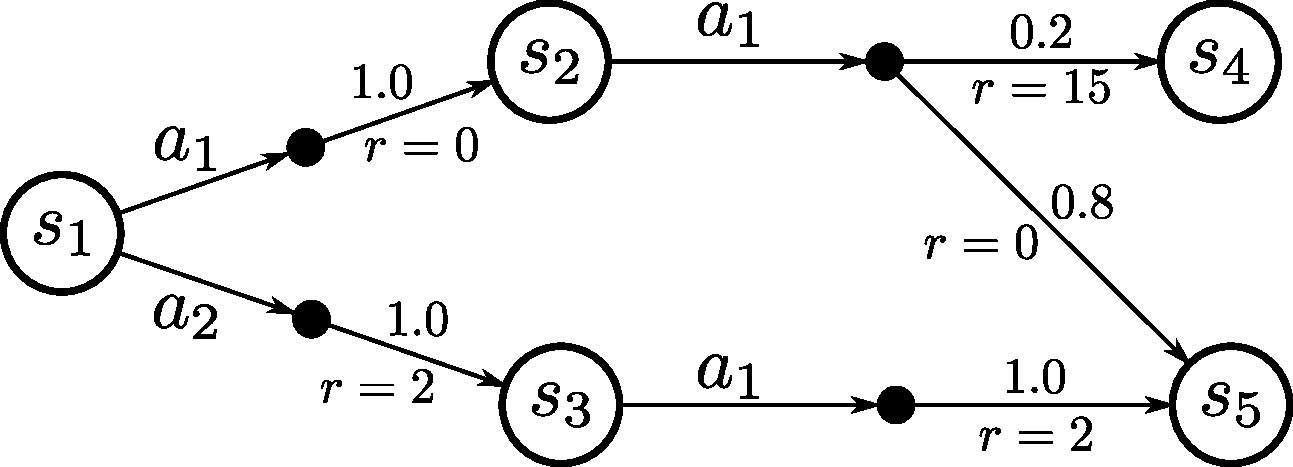
\includegraphics[width=0.8\textwidth]{figures/ch2/example_mdp.pdf} 
        \caption[An example MDP $\cl{M}$.]{An example MDP $\cl{M}$, where $s_0=s_{\cl{M}}^1$, the finite horizon is $H=2$, and terminal states are marked with a thicker border. Edges are appropriately marked with actions and rewards, or marked with transition probabilities.}
        \label{fig:2:mdp_eg}
    \end{figure}

    An example MDP is shown in Figure \ref{fig:2:mdp_eg}. Notationally, it is convenient to define the set of successor states, that is the set of states that could be reached after taking an action from the current state of the MDP:
    \begin{defn}
        \label{def:2:succ}
        The set of \textnormal{successor states} $\suc{s}{a}$ of a state-action pair $(s,a)$, with respect to an MDP, is defined as: 
        \begin{align}
            \suc{s}{a}:=\{s'\in\cl{S}|p(s'|s,a)>0\}. \label{eq:2:succ_def}
        \end{align}
    \end{defn}

    Additionally, throughout this thesis, MDPs will be defined with \textit{terminal states}, which are states that once reached will never be left, and no more reward can be obtained. 
    \begin{defn}
        \label{def:2:terminal}
        A state $s\in\cl{S}$ is a \textnormal{terminal} state (or a \textnormal{trap} state), if the transition distribution always returns the same state (i.e. $p(s|s,a)=1$ for all actions $a$), and if no more reward is obtained from that state ($R(s,a)=0$ for all $a$). The function $\terminal(s)$ returns a boolean in $\{\textnormal{True},\textnormal{False}\}$ which will be used to denote if a state $s$ is terminal or not.
    \end{defn}

    To define a strategy that an agent will follow in an MDP, and agent defines a \textit{policy}. A policy maps each state in the state space to a probability distribution over the action space. To ``follow'' a policy, actions are sampled from the distribution. Often it is desirable to define deterministic policies, which always produce the same action when given the same state, and can be represented as \textit{one-hot} distributions. 

    \begin{defn}
        \label{def:2:policy}
        A \textnormal{(stochastic) policy} $\pi:\cl{S}\rightarrow (\cl{A} \rightarrow [0,1])$ is a mapping from states to a probability distributions over actions and $\pi(a|s)$ is the probability of sampling action $a$ at state $s$. The policy $\pi$ must satisfy the conditions: for all $s \in \cl{S}$ we have $\sum_{a\in\cl{A}} \pi(a|s) = 1$ and for all actions $a\in\cl{A}$ that $\pi(a|s)\geq 0$ . 
        
        Additionally, a \textnormal{deterministic policy} is defined as a one-hot policy, that is, the policy $\pi$ is deterministic iff it can be written as $\pi(a|s)=\one[a=a']$ for some $a'\in\cl{A}$.

        Moreover, the following notations are used for policies:
        \begin{itemize}
            \item $a\sim\pi(\cdot|s)$ denotes sampling an action $a$ from the distribution $\pi(\cdot|s)$;
            \item $\pi(s)=a'$ is used as a shorthand to define the deterministic policy $\pi(a|s)=\one[a=a']$; 
            \item $\pi(s)$ is used as a shorthand for the action $a'\sim\pi(\cdot|s)$ in the case of a deterministic policy.
        \end{itemize}
    \end{defn}
    
    Given an MDP $\cl{M}$ and a policy $\pi$ it is then possible to sample a sequence of states, actions and rewards, known as a \textit{trajectory}. A trajectory \textit{simulates} one possible sequence that could occur if an agent follows policy $\pi$ in $\cl{M}$, and in Section \ref{sec:2-4-thts} these simulations are used to incrementally build a search tree.
    
    \begin{defn}
        \label{def:2:trajectory}
        A \textnormal{trajectory} $\tau$, is a sequence of state, action and rewards, that is induced by a policy $\pi$ and MDP $\cl{M}$ pair. Let the trajectory be $\tau = (s_0, a_0, r_0, s_1, a_1, r_1, ..., s_{H-1}, a_{H-1}, r_{H-1}, s_H)$, where $a_t \sim \pi(\cdot|s_t)$, $r_t=R(s_t,a_t)$ and $s_{t+1} \sim p(\cdot|s_t,a_t)$. 
        
        The following notations will also be used for trajectories:
        \begin{itemize}
            \item $\tau\sim\pi$ denotes a trajectory that is sampled using the policy $\pi$, where the MDP $\cl{M}$ is implicit;
            \item $\tau_{i:j}$ denotes the \textnormal{truncated trajectory} $\tau_{i:j}:=(s_i, a_i, r_i, s_{i+1}, ..., s_{j-1}, a_{j-1}, r_{j-1}, s_j)$, between the timesteps $0\leq i < j \leq H$ inclusive;
            \item $\tau_{:j}:=\tau_{0:j}$ denotes a trajectory that is trunacted on only one end,
            \item given a trajectory $\tau$, the following set notation is used, $s\in \tau$, $(s,a)\in\tau$ as a shorthand for $s\in\{s_i|i=0,...,H\}$ and $(s,a)\in\{(s_i,a_i)|i=0,...,H-1\}$ respectively, 
        \end{itemize}
        and finally, when states, actions and rewards a timestep indexed (i.e. $s_t,a_t,r_t$), they will always correspond to a trajectory.
    \end{defn}







\section{Reinforcement Learning}
\label{sec:2-3-rl}

    \begin{figure}
        \centering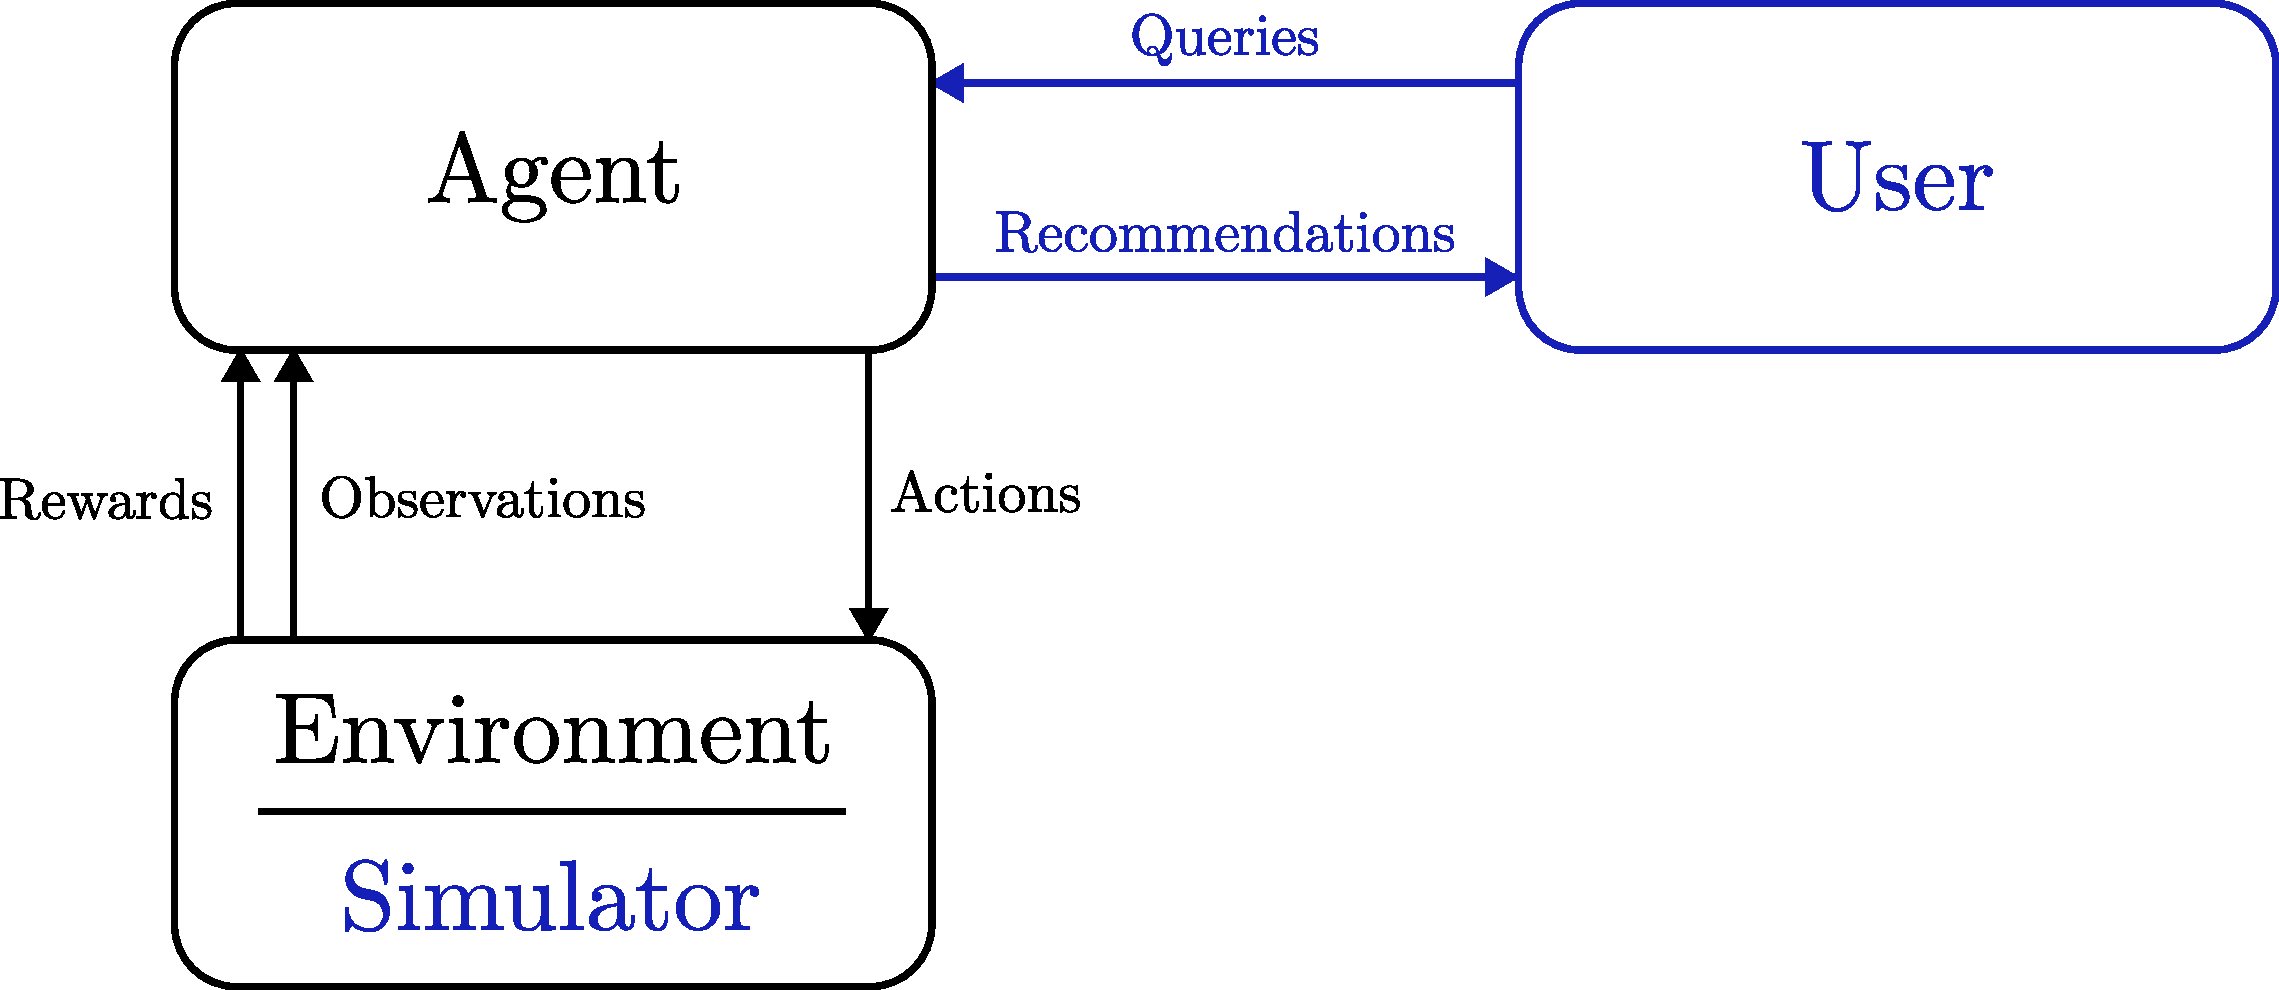
\includegraphics[width=0.75\textwidth]{figures/ch2/rl_overview.pdf} 
        \caption[An overview of reinforcement learning.]{An overview of reinforcement learning. In black depicts the standard agent-environment interface for reinforcement learning \cite{sutton}, where an agent can perform actions in an environment and is given feedback in the form of observations and rewards. In blue the environment is replaced by a simulated environment which the agent can use for planning, and is queried by a user for recommendations on how to act in the real environment.}
        \label{fig:2:rl_overview}
    \end{figure}

    This section serves as a brief introduction to fundamental concepts in reinforcement learning, and motivates an alternative lens on reinforcement learning that this thesis will consider. The field of reinforcement learning considers an agent that has to learn how to make decisions by interacting with its environment (Figure \ref{fig:2:rl_overview}). The agent can take actions in the environment, recieving in return \textit{observations} and \textit{rewards}, which can be used to update internal state and used to make further decisions, and the goal of the agent is to maximise the rewards that it recieves.

    Classically the agent is considered to interact with its environment directly \cite{sutton}, and thus must make a trade-off between exploring new strategies and exploiting learned strategies. That is, reinforcement learning agents must consider the \textit{exploration-exploitation trade-off} discussed in Section \ref{sec:2-1-mab} too. 
    %If an agent were to try to only exploit, then it may not discover better strategies, and if an agent only explores, then it may miss out on the opportunity to exploit the best known strategy and obtain greater rewards.

    Also depicted in Figure \ref{fig:2:rl_overview} is a scenario where the agent is equiped with a simulator that it can use to plan and explore, and is either asked to recommend a strategy after a planning/learning phase, or is occassionally queried to recommend actions. This scenario more closely resembles how reinforcement learning is used in the modern era with greater amounts of compute power available, and interactions with the simulator occur at orders of magnitude quicker. Hence, in this scenario, the only significant real-world cost comes from following the recommendations output, to be used in the real-world environment. This changes the nature of the exploration-exploitation trade off, almost separating the two issues, where there is an emphasis on exploring during the planning phase, and the problem of providing good recommendations is concerned with pure exploitation. This perspective on reinforcement learning motivates the research quesitons around exploration: \exploreq. 

    In this thesis, the environment will always take the form of an MDP (Defintion \ref{def:2:mdp}), and observations will always be \textit{fully-observable}, meaning that the agent is provided with full access to the states of the MDP. 

    Following on from Section \ref{sec:2-2-mdps}, the remainder of this section defines \textit{value functions} and the objectives of reinforcement learning and covers \textit{Value Iteration}, a tabular dynamic programming approach to reinforcement learning. Finally Section \ref{sec:2-3-1-merl} covers \textit{maximum-entropy reinforcement learning}.
    
    The value of a policy $\pi$ is the expected cumulative reward that will be obtained by following the policy:
    \begin{defn}
        \label{def:2:value}
        \label{def:2:q_value}
        The \textnormal{value} of a policy $\pi$ from state $s$ at time $t$ is:
        \begin{align}
            V^{\pi}(s;t) = \bb{E}_{\tau\sim\pi}\left[\sum_{i=t}^{H-1} r_t \Bigg| s_t=s \right]. \label{eq:2:value_fn_def}
        \end{align} 

        The \textnormal{Q-value} of a policy $\pi$, from state $s$, with action $a$, at time $t$ is:
        \begin{align}
            Q^{\pi}(s,a;t) = R(s,a) + \bb{E}_{s'\sim p(\cdot|s,a)} [V^{\pi}(s';t+1)]. \label{eq:2:q_value_fn_def}
        \end{align} 
    \end{defn}

    From the definition of the values functions the optimal value functions can be defined by taking the maximum value over all policies:
    \begin{defn}
        \label{def:2:optimal_value}
        \label{def:2:optimal_q_value}
        The \textnormal{Optimal (Q-)Value} of a state(-action pair) is defined as:
        \begin{align}
            V^*(s;t) &= \max_{\pi} V^{\pi}(s;t) \label{eq:2:opt_value_fn_def} \\
            Q^*(s,a;t) &= \max_{\pi} Q^{\pi}(s,a;t). \label{eq:2:opt_q_value_fn_def}
        \end{align}
    \end{defn}

    Value functions can also be used to define an objective function:
    \begin{defn}
        \label{def:2:rl_obj_fn}
        The \textnormal{(standard) reinforcement learning objective function} $J(\pi)$ is defined as:
        \begin{align}
            J(\pi) = V^{\pi}(s_0;0). \label{eq:2:rl_obj_fn_def}
        \end{align}

        The objective of (standard) reinforcement learning can then be stated as finding $\max_{\pi} J(\pi)$.
    \end{defn}

    The \textit{optimal policy} is the policy that maximises the objective function $J$, and can be shown to be deterministic \cite{kolobov}:
    \begin{defn}
        \label{def:2:opt_policy}
        The \textnormal{optimal (standard) policy} $\pi^*$ is the policy maximising the standard objective function:
        \begin{align}
            \pi^* = \argmax_\pi J(\pi) \label{eq:2:opt_policy_def}
        \end{align}
        or equivalently, the optimal standard policy can be in terms of the optimal Q-value function:
        \begin{align}
            \pi^*(s) = \argmax_a Q^*(s,a). \label{eq:2:opt_policy_from_opt_q_value}
        \end{align}
    \end{defn}

    It can be shown that the optimal (Q-)value functions satisfy the \textit{Bellman equations} \cite{dp,kolobov}:
    \begin{align}
        V^*(s;t) &= \max_{a\in\cl{A}} Q^*(s,a;t), \label{eq:2:bellman_opt_v} \\
        Q^*(s,a;t) &= R(s,a) + \bb{E}_{s'\sim p(\cdot|s,a)} [V^*(s';t+1)]. \label{eq:2:bellman_opt_q}
    \end{align} 

    The Bellman equations admit a \textit{dynamic programming} approach which can be used to computer the optimal value functions, known as \textit{Value Iteration} \cite{dp,kolobov}. In Value Iteration, a table of value estimates $\hat{V}(s;t)$ are kept for each $s,t$. Given any initial estimate of the value function $\hat{V}^{0}$, the \textit{Bellman backup} operations are:
    \begin{align}
        \hat{V}^{k+1}(s;t) &= \max_{a\in\cl{A}} \hat{Q}^{k+1}(s,a;t), \label{eq:2:value_iter_v_backup} \\
        \hat{Q}^{k+1}(s,a;t) &= \bb{E}_{s'\sim p(\cdot|s,a)} [R(s,a) + \hat{V}^k(s';t+1)]. \label{eq:2:value_iter_q_backup}
    \end{align}

    In each iteration of Value Iteration, these values are computed for all $s\in\cl{S}$, $a\in\cl{A}$ and $t\in\{0,1,...,H\}$. The value estimates computed from the Bellman backups will converge to the optimal values in a finite number of iterations: $V^{k}\rightarrow V^*$.









    \subsection{Maximum Entropy Reinforcement Learning}
    \label{sec:2-3-1-merl}

        In \textit{maximum-entropy reinforcement learning}, the objective function is altered to include the addition of an entropy term. The addition of an entropy term is motivated by wanting to learn stochastic behaviours, that better explore large state spaces, and learn more robust behaviours under uncertainty by potentially learning multiple solutions rather than a single deterministic solution \cite{deep_energy_policies}. 
        
        Let $\cl{H}$ denote the (Shannon) entropy function \cite{entropy}:
        \begin{align}
            \cl{H}(\pi(\cdot|s)) = \bb{E}_{a\sim\pi(\cdot|s)}[-\log \pi(a|s)] = \sum_{a\in\cl{A}} \pi(a|s) \log \pi(a|s). \label{eq:2:shannon_entropy_def}
        \end{align}

        In the maximum entropy objective, the relative weighting of entropy terms is included using a coefficient $\alpha$, called the \textit{temperature}. In the maximum entropy objective, analogues of the value functions can be defined, which are typically referred to as \textit{soft (Q-)values}, and similarly the maximum entropy objective is often referred to as the \textit{soft objective}.

        \begin{defn}
            \label{def:2:sft_value}
            \label{def:2:sft_q_value}
            The \textnormal{soft value} of a policy $\pi$ from state $s$ at time $t$ is:
            \begin{align}
                V_{\sft}^{\pi}(s;t) = \bb{E}_{\tau\sim\pi}\left[\sum_{i=t}^{H-1} r_t + \alpha\cl{H}(\pi(\cdot|s_i)) \Bigg| s_t=s \right]. \label{eq:2:sft_value_fn_def}
            \end{align} 

            The \textnormal{soft Q-value} of a policy $\pi$, from state $s$, with action $a$, at time $t$ is:
            \begin{align}
                Q_{\sft}^{\pi}(s,a;t) = R(s,a) + \bb{E}_{s'\sim p(\cdot|s,a)} [V_{\sft}^{\pi}(s';t+1)]. \label{eq:2:sft_q_value_fn_def}
            \end{align} 
        \end{defn}

        The optimal soft (Q-)values can be defined by taking the maximum over policies, similarly to the standard objective:
        \begin{defn}
            \label{def:2:optimal_sft_value}
            \label{def:2:optimal_sft_q_value}
            The \textnormal{optimal soft (Q-)Value} of a state(-action pair) is defined as:
            \begin{align}
                V_{\sft}^*(s;t) &= \max_{\pi} V_{\sft}^{\pi}(s;t), \label{eq:2:opt_soft_value_fn_def} \\
                Q_{\sft}^*(s,a;t) &= \max_{\pi} Q_{\sft}^{\pi}(s,a;t). \label{eq:2:opt_soft_q_value_fn_def}
            \end{align}
        \end{defn}

        In maximum entropy reinforcement learning, the objective is to find a policy with maximal soft value.
        \begin{defn}
            \label{def:2:soft_rl_obj_fn}
            The \textnormal{maximum entropy (or soft) reinforcement learning objective function} $J_{\sft}(\pi)$ is defined as:
            \begin{align}
                J_{\sft}(\pi) = V_{\sft}^{\pi}(s_0;0). \label{eq:2:soft_rl_obj_fn_def}
            \end{align}

            The objective of maximum entropy (or soft) reinforcement learning can then be stated as finding $\max_{\pi} J_{\sft}(\pi)$.
        \end{defn}

        The optimal soft policy is defined as the policy that maximises the soft objective function $J_{\sft}$, and it can be computed from the optimal soft (Q-)values.
        \begin{defn}
            \label{def:2:opt_sft_policy}
            The \textnormal{optimal soft policy} $\pi_{\sft}^*$ is the policy maximising the soft objective function:
            \begin{align}
                \pi_{\sft}^* = \argmax_\pi J_{\sft}(\pi). \label{eq:2:opt_sft_policy_def}
            \end{align}
            Given $V_{\sft}^*$ and $Q_{\sft}^*$ the optimal soft police is known to take the form \cite{deep_energy_policies}:
            \begin{align}
                \pi_{\sft}^*(a|s;t) = \exp\left(\left(Q_{\sft}^*(s,a;t) - V_{\sft}^*(s;t)\right) / \alpha \right). \label{eq:2:opt_sft_policy_from_opt_value_fns}
            \end{align}
        \end{defn}

        Equations similar to the Bellman equations, aptly named the \textit{soft Bellman equations}, can be defined for maximum entropy reinforcement learning. These equations differ to equations (\ref{eq:2:bellman_opt_v}) and (\ref{eq:2:bellman_opt_q}) by the replacement of the $\max$ operation with a \textit{softmax} or \textit{log-sum-exp} operation, and explain why the maximum entropy analogues are referred to as the \textit{soft} versions of their standard reinforcement learning counterparts. The \textit{soft Bellman equations} are \cite{deep_energy_policies}:
        \begin{align}
            V_{\sft}^*(s;t) &= \alpha \log \sum_{a\in\cl{A}} \exp\left( Q_{\sft}^*(s,a;t) / alpha \right), \label{eq:2:sft_bellman_opt_v} \\
            Q_{\sft}^*(s,a;t) &= R(s,a) + \bb{E}_{s'\sim p(\cdot|s,a)} [V_{\sft}^*(s';t+1)]. \label{eq:2:sft_bellman_opt_q}
        \end{align} 

        Analogous to standard reinforcement learning, the soft Bellman equations can be used in \textit{soft Bellman backups} for a \textit{Soft Value Iteration} algorithm \cite{deep_energy_policies}:
        \begin{align}
            \hat{V}_{\sft}^{k+1}(s;t) &= \alpha \log \sum_{a\in\cl{A}} \exp\left( \frac{1}{\alpha} \hat{Q}_{\sft}^{k+1}(s,a;t) \right), \label{eq:2:soft_value_iter_v_backup} \\
            \hat{Q}_{\sft}^{k+1}(s,a;t) &= R(s,a) + \bb{E}_{s'\sim p(\cdot|s,a)} [\hat{V}_{\sft}^k(s';t+1)]. \label{eq:2:soft_value_iter_q_backup}
        \end{align}

        














\section{Trial-Based Heuristic Tree Search and Monte Carlo Tree Search}
\label{sec:2-4-thts}

    \begin{figure}
        \centering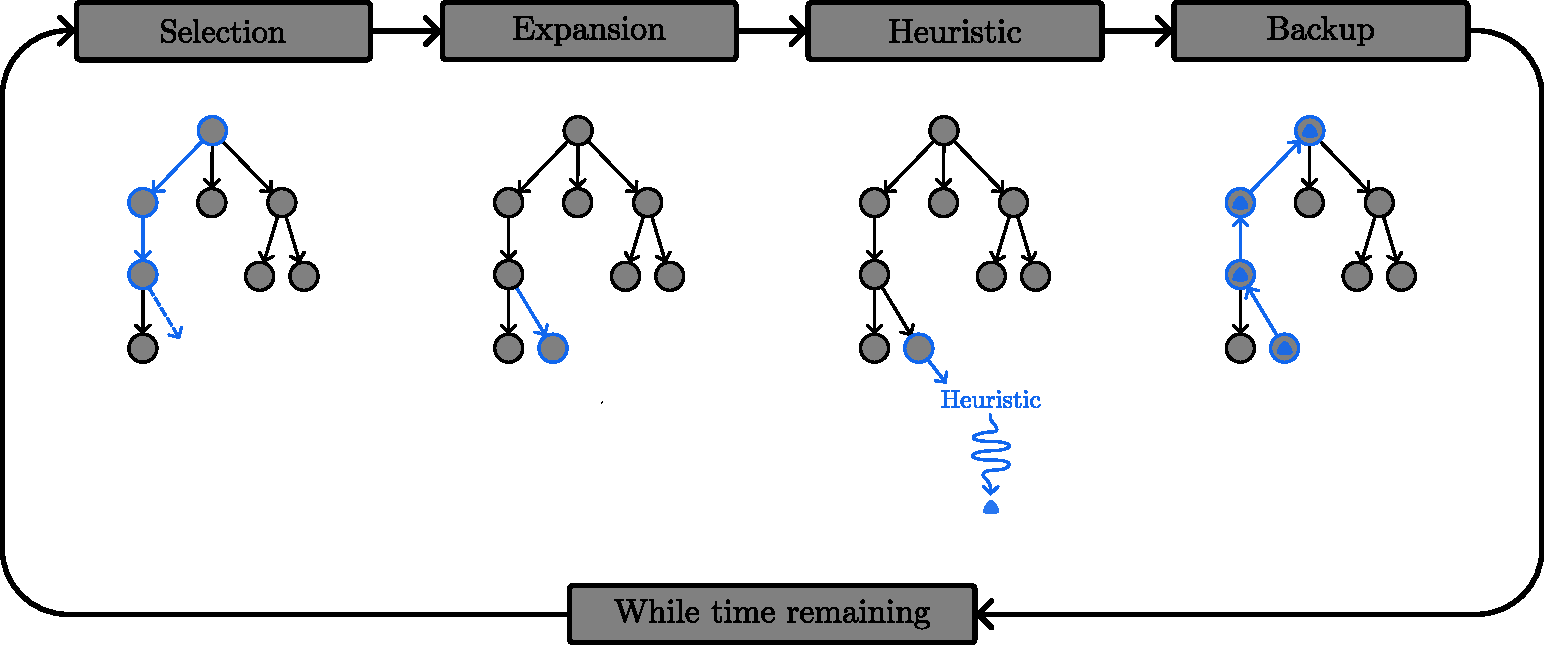
\includegraphics[width=1.0\textwidth]{figures/ch2/mcts_trial.pdf} 
        \caption[Overview of one trial of \mctsone.]{Overview of one trial of \mctsone, depicting the four commonly presented stages \cite{mcts_survey}. First, in the selection phase a search policy is used to sample a path down the tree. Next a new node is added to the search tree. Then the new node is initialised using a heuristic, often using a \textit{simulation} using a \textit{rollout policy} as depicted. Finally, values (triangles) are updated through \textit{backups} along the path sampled in the selection phase.}
        \label{fig:2:mcts}
    \end{figure}

    When considering MDPs with large state-action spaces, using tabular dynamic programming methods becomes infeasibly slow. One approach for handling large state-action spaces is to use \textit{heuristic methods}, that consider a subset of the state-action space and utilise heuristic estimates for the value of states. Often these heuristic methods build a \textit{search tree} from the initial state of the MDP.

    Monte Carlo Tree Search (MCTS) refers to heuristic algorithms that build a search tree using \textit{Monte Carlo Trials}, where nodes are added to the tree based off randomly sampled trajectories. Two advantages of using MCTS methods in the modern day are: that they allow for statistical analysis, which can provide \textit{probabilistic guarantees} for the performance of the algorithm; and they offer interpretability, as the search tree can be inspected post-hoc to identify why the algorithm made certain decisions. \hide{\todo{consider adding interperobility refs when litrev'ed}}

    MCTS trials are commonly presented using four stages, selection, expansion, simulation/heuristic and backup phases \cite{mcts_survey}, which are depicted in Figure \ref{fig:2:mcts}. To avoid confusion with the above definition of MCTS, this thesis will refer to this specific form of MCTS as \mctsone. Each of the four phases of \mctsone\ewe are described in more detail below: 
    \begin{enumerate}
        \item \textit{Selection phase} - a \textit{search policy} is used to traverse the search tree from the root node until it reaches a state not contained in the search tree;
        \item \textit{Expansion phase} - a new child node is added to the search tree;
        \item \textit{Simulation/Heuristic phase} - the new child node's value is initialised using a \textit{heuristic}, often taking the form of a Monte Carlo return, obtained using a \textit{simulation} with a \textit{rollout policy}; 
        \item \textit{Backup phase} - the value from the heuristic or simulation is used to backup values through the path traversed in the selection phase.
    \end{enumerate}

    Trial-Based Heuristic Tree Search (THTS) \cite{thts} generalises heuristic tree search methods used for planning, such as Trial-Based Real Time Dynamic Programming \cite{rtdp} and LAO$^*$ \cite{lao_star}. However, THTS differs slightly from how \mctsone\ewe is presented above. In a THTS trial, after the expansion/heurisitc phases are run, the trial ``switches back to the selection phase and alternate between those phases'', until the planning horizon is reached. This is similar to the trial depicted in blue in Figure \ref{fig:2:thts}.

    \thtspp\ewe \cite{thtspp} is introduced in Section \ref{sec:2-4-1-thts}, which is an open-source, parallelised extension of the THTS schema (including being able to implement \mctsone\ewe algorithms), and was built to facilitate the work in this thesis. Section \ref{sec:2-4-2-uct} covers the Upper Confidence Bound applied to Trees (UCT) algorithm \cite{uct,uct_long}, which is a commonly used MCTS algorithm, and Section \ref{sec:2-4-3-ments} presents the Maximum ENtropy Tree Search (MENTS) algorithm \cite{ments}, which is related to the algorithms introduced in Chapter \ref{ch:4-dents} of this thesis.
    
    


    




    \subsection{Notation}
    \label{sec:2-4-0-notation}
        To simplify notation in the presentation and analysis of \thtspp\ewe algorithms, this thesis assumes that states and state-action pairs have a one-to-one correspondance with nodes in the search tree. This assumption is purely to simplify notation for a clean presentation, and any results discussed in this thesis generalise to when this assumption does not hold. 

        Specifically, this allows the notation for value functions to avoid explicitly writing the timestep parameter, so that $V^{\pi}(s)$ can be written instead of $V^{\pi}(s;t)$.






    \subsection{Trial Based Heuristic Tree Search}
    \label{sec:2-4-1-thts}

        This subsection introduces \thtspp\ewe, which extends the Trial-Based Heuristic Tree Search (THTS) schema \cite{thts}, and aims to provide a modular library which can implement any MCTS algorithm. The changes made to the original schema allow algorithms following the four-phase \mctsone\ewe trials described previously to be encorporated. Additionally, the notion of a per-trial \textit{context} is added, which will be used in Chapters \ref{ch:5-chmcts} and \ref{ch:6-simplexmaps} for multi-objective MCTS algorithms. Additionally, beyond the scope of this thesis, contexts allow \thtspp\ewe to implement algorithms for \textit{partially-observable} environments, such as Partially Observable Monte Carlo Planning \cite{pomcp}. The remainder of this section will be presented in the context of planning for fully-observable MDPs, but \thtspp\ewe generalises to partially-observable environments if \textit{observation-action histories} are used in place of states.

        In \thtspp\ewe trees consist of \textit{decision nodes} and \textit{chance nodes}. Decision nodes sample actions that can be taken by the agent, and chance nodes sample \textit{outcomes} (MDP states) that depend on the action taken and the transition function of the MDP. As such, each decision node has an associated \textit{state} and each chance node has an associated \textit{state-action pair}. Figure \ref{fig:2:tree_notation} shows how decision and chance nodes will be depicted as circles and diamonds in diagrams.

        \begin{figure}
            \centering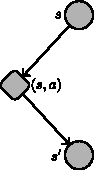
\includegraphics[width=0.2\textwidth]{figures/ch2/tree_notation.pdf} 
            \caption[Tree diagrams notation.]{Tree diagrams notation, circles will be used to denote \textit{decision nodes} that are associated with states, diamonds will be used to denote \textit{chance nodes} that are associated with state-action pairs and arrows are used to denote parent/child relationships in the tree.}
            \label{fig:2:tree_notation}
        \end{figure}

        A search tree $\cl{T}$ is built using Monte Carlo \textit{trials} and an overview of one trial in \thtspp\ewe is given in Figure \ref{fig:2:thts}. Each \thtspp\ewe trial is also split into four phases: 
        \begin{enumerate}
            \item  
                \textit{Context sampling} - a \textit{context} is sampled for the trial;
            \item 
                \textit{Selection phase} - a trajectory is sampled using a \textit{search policy}, any newly visited states (and state-action pairs) are added to $\cl{T}$ as decision nodes (and chance nodes);
            \item 
                \textit{Heuristic phase} - any new leaf nodes added in the selection phase are initialised using a \textit{heuristic function}; 
            \item 
                \textit{Backup phase} - value estimates in the search tree are updated, along the path sampled in the selection phase. 
        \end{enumerate}

        Note that the selection and expansion phases of \mctsone\ewe are encapsulated by the selection phase of \thtspp.

        \begin{figure}
            \centering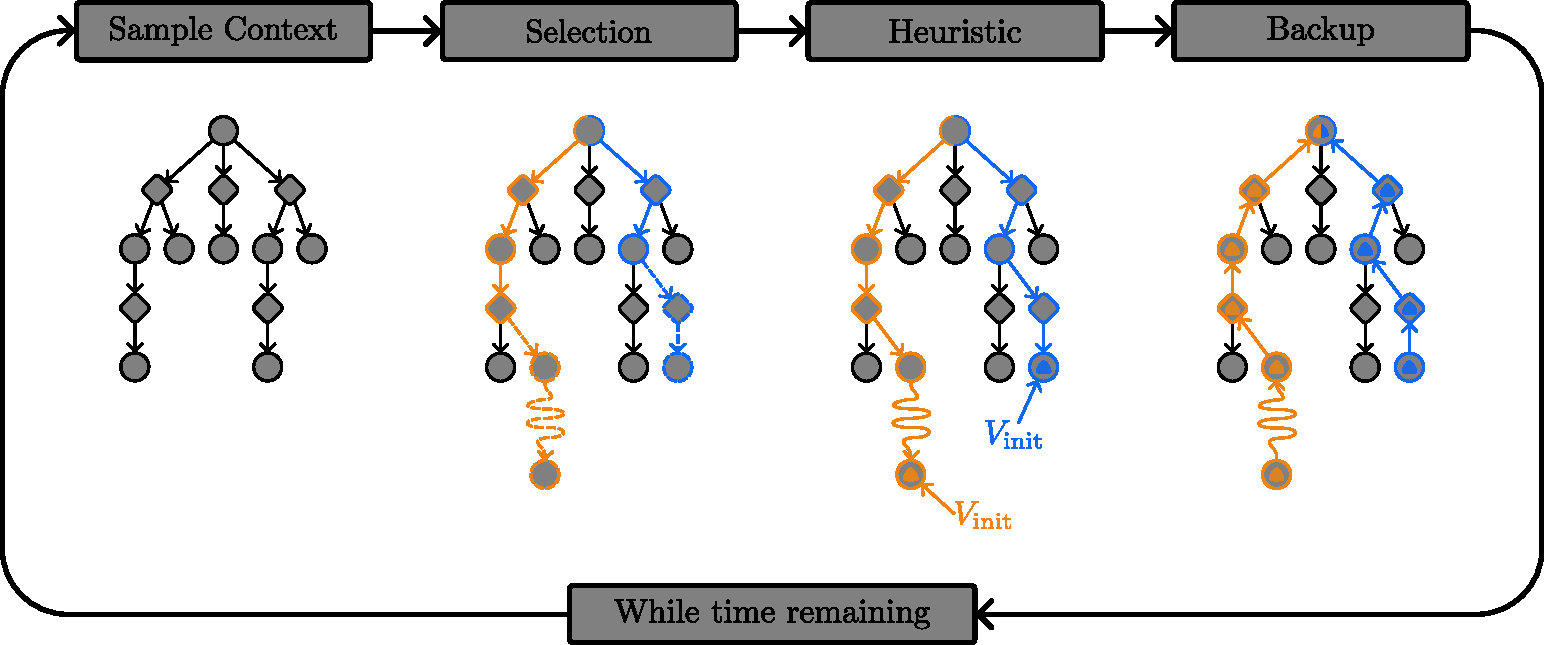
\includegraphics[width=1.0\textwidth]{figures/ch2/thts_trial.pdf} 
            \caption[Overview of one trial of \thtspp.]{Overview of one trial of \thtspp, where orange shows an example when \mctsmode\ewe is True, and blue shows an example when \mctsmode\ewe is False. From left to right: first a context is sampled, which stores any necessary per-trial state (not depicted) and the search tree at the beginning of the trial is shown; second shows the selection phase, where a trajectory is sampled and where dashed lines indicate any new nodes added; third shows that new leaf nodes are initialised using the $\Vinit$ heuristic function; and finally on the right, shows the backup phase, where the arrows directions are changed to show that information is being propogated back up the tree to update the values in the nodes (triangles).}
            \label{fig:2:thts}
        \end{figure}

        \begin{defn}
            \label{def:2:search_tree}
            A \textnormal{search tree} $\cl{T}$ is a subset of the state and state-action spaces, that is $\cl{T}\subseteq \cl{S} \cup \cl{S} \times \cl{A}$, where for each $s\in\cl{T}$, there exists some truncated trajectory $\tau_{:h}$ such that $s_h = s$, each $s'\in\tau_{:h}$ is also in the tree, $s'\in\cl{T}$, and each $s',a'\in\tau{:h}$ is also in the tree, $(s',a')\in\cl{T}$.
        \end{defn}

        % \begin{defn}
        %     \label{def:2:cnode}
        %     \label{def:2:dnode}
            A \textit{decision node} refers to any state that is in the search tree: $s\in\cl{T}$. A \textit{chance node} refers to any state-action pair that is in the search tree: $(s,a)\in\cl{T}$. And a \textit{node} is used to refer to any decision or chance node in the tree. Sometimes the notation $\node(s)$ and $\node(s,a)$ will be used to make it clear that a node is being discussed, rather than a state or state-action pair.

            $N(s)$ and $N(s,a)$ denote the number of times $\node(s)$ and $\node(s,a)$ have been visited, or equivalently, the number of times $s$ and $(s,a)$ appear in trajectories sampled in \thtspp\ewe trials.

            Each decision and chance node will generally store value estimates that are algorithm dependent. $\dnodedata{s}$ is used to denote the set of values stored at node $\node(s)$, and $\cnodedata{s,a}$ for the set of values stored at node $\node(s,a)$. 

            Additionally, let $\node(s)\dotchildren$ be a mapping from actions to the chance nodes that are children of $\node(s)$. Likewise, $\node(s,a)\dotchildren$ is a mapping from outcomes (successor states) to the decision nodes that are children of $\node(s,a)$.
        % \end{defn}

        \thtspp\ewe introduces the idea of \mctsmode\ewe into the THTS schema. When \mctsmode\ewe is True, a single decision node is added to the search tree on each trial, similarly to \mctsone. When it is False, the trajectory is sampled until a terminal state or the planning horizon is reached. These two modes of operation are depicted in blue and orange respectively in Figure \ref{fig:2:thts}.
        \begin{defn}
            \label{def:2:mctsmode}
            When running in \mctsmode, the trajectory sampled in the selection phase is truncated, and will end if a state not in the search tree $\cl{T}$ is reached, similarly to \mctsone\ewe \cite{mcts_survey}. When not running in \mctsmode, the trajectory is sampled until a terminal state is reached, or the planning horizon is reached, similarly to THTS \cite{thts}. 
        \end{defn} 

        There are two main benefits to running an algorithm in \mctsmode. The first is that it uses significantly less memory, which can be a concern if using a large planning horizon $H$ and the tree search is going to run for a long time. The second is that if \mctsmode\ewe is used with an informative heuristic function, then it allows the algorithm to avoid wasting resouces (time and memory) on parts of the search tree that are not promising. 
        
        In contrast, when no informative heuristic is available, a random simulation is often used in \mctsone\ewe algorithms. In such cases, where memory allows, running with \mctsmode\ewe set to False can be beneficial, because states that would have been visited in the simulation phase of \mctsone\ewe are added to the tree and avoids throwing away potentially useful information.

        \thtspp\ewe also introduces the notion of a \textit{context} that is sampled for each trial. The context is passed to every subsequent function call in a trial of \thtspp, and can be used to store temporary state. This context will go unused for the remainder of the chapter, but will be useful in Chapters \ref{ch:5-chmcts} and \ref{ch:6-simplexmaps} when \textit{contextual tree search} is discussed.
        \begin{defn}
            \label{def:2:thts_context}
            A \textnormal{context} is an arbitrary key-value store that is used to store any relevant data that varies from trial to trial.
        \end{defn}  

        To specify an algorithm in the \thtspp\ewe schema, the following need to be specified:
        \begin{description}
            \item[Value Estimates:]
                What value estimates will be stored at each decision and chance node. That is, $\dnodedata{s}$ and $\cnodedata{s,a}$ need to be defined;
            \item[Search policy:]
                A policy $\pisearch$ used to sample a trajectory for the trial, which can use values in the current search tree $\cl{T}$, and values from the heuristic action function (below);
            \item[Outcome Sampler:]
                A function \sampleoutcome\ewe that samples outcomes according to the environment, given a current state and action. In this thesis, this will always sample a state from the transition distribution of the MDP: $s'\sim p(\cdot|s,a)$;
            \item[Heuristic value function:]
                A function $\Vinit$ used as a heuristic to initialise values for new decision nodes added to the tree;
            \item[Heuristic action function:]
                A function $\Qinit$ used as a heuristic for Q-values when a state-action pair is not in the current search tree;
            \item[Backup functions:]
                Two functions $\backupv$ and $\backupq$ which updates the values in decision and chance nodes respectively. These functions can use values from their children, from the sampled trajectory and from the heuristic value function;
            \item[Context sampler:]
                A function $\samplecontext$ which creates a context key-value store, and samples any initial values to be stored in the context;
            \item[MCTS mode:]
                A boolean (which will also be denoted \mctsmode) specifying if \thtspp\ewe should operate in \mctsmode;
            \item[Planning horizon:]
                 A (problem dependent) planning horizon for the tree search $H_{\thtspp}$, which is no longer than the horizon of the MDP, $H_{\thtspp}\leq H$.
        \end{description}
        
        Figure \ref{fig:2:thts} depicts a trial in \thtspp, and psuedocode for running a trial is given in Listing \ref{lst:2:thts_trial}. At the beginning of runnning a \thtspp\ewe algorithm, the search tree is initialised to $\cl{T}\leftarrow\{s_0\}$. When the components detailed above are provided, the operation of a trial in \thtspp\ewe is as follows:
        \begin{itemize}
            \item Firstly, a context is sampled using the $\samplecontext$ function, which is available to be used by any other function in the trial.
            \item A trajectory is sampled $\tau_{:h}\sim\pisearch$ according to the search policy (which may use $\Qinit$ as necessary) and \sampleoutcome.
            \begin{itemize}
                \item If running in \mctsmode, then $\tau_{:h}$ is such that $s_t\in\cl{T}$ for $t=0,...,h-1$ and $s_h\not\in\cl{T}$, or $h=H_{\thtspp}$, or $s_h$ is terminal.
                \item If not running in \mctsmode, then $h=H_{\thtspp}$, or $s_h$ is terminal.
            \end{itemize}
            \item The search tree is updated to include any new nodes from the sampled trajectory, $\cl{T}\leftarrow\cl{T}\cup\tau_{:h}$.
            \item The heuristic value function is used to initialise the value of the new leaf node $\dnodedata{s_h}\leftarrow \Vinit(s_h)$.
            \item Finally, for the backup phase, the $\backupq$ and $\backupv$ functions are used to update the values of $\cnodedata{s_t,a_t}$ and $\dnodedata{s_t}$ for $t=h-1,...,0$.
        \end{itemize}
               
        
        \begin{Listing}
            \begin{lstlisting}
def run_trial(search_tree: $\cl{T}$, 
              search_policy: $\pisearch$, 
              heuristic_fn: $\Vinit$,
              heuristic_action_fn: $\Qinit$,
              mcts_mode,
              planning_horizon: $H_{\thtspp}$):
    # context sampling
    ctx = sample_context()
    # simulation phase
    $\tau_{:h}$ = sample_trajectory($\cl{T}$, $\pisearch$, $\Qinit$, mcts_mode, $H_{\thtspp}$, ctx)
    $\cl{T} \leftarrow \cl{T} \cup \tau_{:h}$
    # heuristic phase
    node$(s_h)$.V $\leftarrow \Vinit(s_h$, ctx$)$
    # backup phase
    for i in $\{h-1,h-2,...,1,0\}$:
        node$(s_i,a_i)$.backup_q(node$(s_i,a_i)\dotchildren$, $\tau_{:h}$, $\Vinit(s_h)$, ctx)
        node$(s_i)$.backup_v(node$(s_i)\dotchildren$, $\tau_{:h}$, $\Vinit(s_h)$, ctx)

def sample_trajectory(search_tree: $\cl{T}$, 
                      search_policy: $\pisearch$, 
                      heuristic_action_fn: $\Qinit$,
                      mcts_mode,
                      planning_horizon: $H_{\thtspp}$,
                      ctx):
    i = 0
    while ((not mcts_mode or $s_{\texttt{i}}\in\cl{T}$) 
           and (i < $H_{\thtspp}$) 
           and (not terminal($s_{\texttt{i}}$)):
        $a_{\texttt{i}} \sim \pisearch(\cdot | s_{\texttt{i}},$ ctx$)$ 
        $r_{\texttt{i}} \leftarrow R(s_{\texttt{i}}, a_{\texttt{i}})$
        $s_{\texttt{i+1}} \leftarrow$ sample_outcome$(s_{\texttt{i}}$, $a_{\texttt{i}}$, ctx$)$
        i += 1
    return $(s_0,a_0,r_0,s_1,...,s_{\texttt{i-1}}, a_{\texttt{i-1}},r_{\texttt{i-1}}, s_{\texttt{i}})$

def sample_outcome($s$, $a$, ctx):
    $s' \sim p(\cdot | s, a)$
    return $s'$
            \end{lstlisting}
            \caption{Psuedocode for running a trial in \thtspp.}
            \label{lst:2:thts_trial}
        \end{Listing}


    



    
    \subsection{Upper Confidence Bounds Applied to Trees (UCT)}
    \label{sec:2-4-2-uct}

        Upper Confidence Bound applied to Trees (UCT) \cite{uct,uct_long} is a commonly used tree search algorithm, which is based on the Upper Confidence Bound (UCB) algorithm covered in Section \ref{sec:2-1-mab}. UCT is a good example of a common paradigm in tree search algorithms for sequential decision making, where each node in the tree is tasked with making a single decision in the sequence, and so adapts methods from the MAB literature. More specifically, UCT can be viewed as running UCB on a non-stationary MAB at every decision node, where it is non-stationary because the rewards obtained depend on the decisions that children make. The remainder of this subsection will outline how UCT can be defined using the the \thtspp\ewe schema given in Section \ref{sec:2-4-1-thts}.

        In UCT \mctsmode\ewe is set to True. And at each decision and node of UCT a sample average $\Vuct$ and $\Quct$ is used for a value estimate. The search policy that UCT then follows is given by:
        \begin{align}
            \piuct(s) = \argmax_{a\in\cl{A}} \Quct(s,a) + b_{\uct} \sqrt{\frac{\log(N(s))}{N(s,a)}}, \label{eq:2:uct_policy}
        \end{align}
        where $b_{\uct}$ is a \textit{bias} parameter that controls the amount of exploration UCT will perform. In Equation (\ref{eq:2:uct_policy}), when $N(s,a)=0$ there is a division by zero, which is taken as $\infty$, and ties are broken uniformly randomly. Note that like UCB (Section \ref{sec:2-1-mab}), this results in every action being taken once to obtain an initial value estimate, and as such, setting $\Qinit$ is unnecessary for UCT.   
        
        There are two common approaches to implementing $\Vinit$ in UCT: the first consisting of using a function approximation $\tilde{V}$ and setting $\Vinit=\tilde{V}$ \cite{alpha_go_zero,alpha_zero,a0c} \hide{\todo{find another paper or two that is just an application of alphazero?}}, where $\hat{V}$ aims to approximate the optimal value function $V^*$; the second approach consists of using a \textit{rollout policy} \cite{mcts_survey,rave,prost,bus}. When a rollout policy $\pirollout$ is used, a Monte Carlo estimate $\hat{V}^{\pirollout}$ is used to estimate the value function $V^{\pirollout}$ and is used for $\Vinit$.

        Let $\tau_{:h}\sim\piuct$, be the trajectory sampled in the selection phase of UCT, meaning that a decision node for $s_h$ is added to the search tree, and needs to be initialised with $\Vinit$. When using a rollout policy, the truncated trajectory is completed using the rollout policy, $\tau_{h:H}\sim\pirollout$, to provide the Monte Carlo estimate at $s_h$:
        \begin{align}
            \hat{V}^{\pirollout}(s_h) = \sum_{i=h}^{H-1} r_i. \label{eq:2:rollout_value_estimate}
        \end{align}

        If no informative policy is available to be used for $\pirollout$, then uniformly random policy is often used \cite{mcts_survey,rand_mc_est_orig}.

        In UCT the backups $\backupv$ and $\backupq$ update the (sample average) value estimates. Letting heuristic value for the leaf node be $\tilde{r} = \Vinit(s_h)$, they are computed as follows:
        \begin{align}
            \Quct(s_t,a_t) &\leftarrow 
                \frac{1}{N(s_t,a_t)} \left( (N(s_t,a_t)-1) \Quct(s_t,a_t) 
                    + \tilde{r} + \sum_{i=t}^{h-1} r_i \right) \label{eq:2:uct_backup_q} \\
            \Vuct(s_t) &\leftarrow 
                \frac{1}{N(s_t)} \left( (N(s_t)-1) \Vuct(s_t,a_t) 
                    + \tilde{r} + \sum_{i=t}^{h-1} r_i \right) \label{eq:2:uct_backup_v} 
        \end{align}  








    \subsection{Maximum Entropy Tree Search}
    \label{sec:2-4-3-ments}

        Maximum ENtropy Tree Search (MENTS) \cite{ments}, in contrast to UCT, focuses on the maximum-entropy objective, and uses soft Bellman backups to update its value estimates. In its original presentation \mctsmode\ewe is set to True, and it uses the soft value estimates $\Vments$ and $\Qments$. The MENTS search policy is given by:
        \begin{align}
            \piments(a|s) &= 
                (1-\lambda_s)\exp\left(\frac{1}{\alpha_{\ments}}\left(\Qments(s,a)-\Vments(s)\right)\right) 
                    + \frac{\lambda_s}{|\cl{A}|}, \label{eq:2:ments_policy}
        \end{align}
        where $\lambda_s=\min(1,\epsilon/\log(e+N(s))),$ with $\epsilon \in (0,\infty)$ is an exploration parameter, and $\alpha_{\ments}$ is the temperature paramter used in MENTS for the maximum entropy objective (the coefficient of the entropy term in Equation (\ref{eq:2:sft_value_fn_def})).

        In MENTS the backups $\backupv$ and $\backupq$ update the soft value estimates and are updated using soft Bellman backups (Equations (\ref{eq:2:soft_value_iter_v_backup}) and (\ref{eq:2:soft_value_iter_q_backup})) as follows:
        \begin{align}
            \Qments(s_t,a_t) &\leftarrow 
                R(s_t,a_t) + \sum_{s'\in\suc{s}{a}} \left( \frac{N(s')}{N(s_t,a_t)} \Vments(s') \right), \label{eq:2:ments_backup_q} \\
            \Vments(s_t) &\leftarrow 
                \alpha \log \sum_{a\in\cl{A}} \exp \left(\frac{1}{\alpha}\Qments(s_t,a) \right). \label{eq:2:ments_backup_v} 
        \end{align}

        In \cite{ments}, the heuristic value function left as an arbitrary evaluation function, but is set using a function approximation $\Vinit=\tilde{V}$ in experiments. The heuristic action function is set to zero, $\Qinit(s,a)=0$, but they also suggest that if \textit{policy network} $\tilde{\pi}$ is available, then the heuristic action function can alternatively be set to $\Qinit(s,a)=\log \tilde{\pi}(s|a)$. 















\section{Multi-Objective Reinforcement Learning}
\label{sec:2-5-morl}

    This thesis follows a utility based approach to multi-objective reinforcement learning similar to the review of \citet{morl_survey}. This work will specifically consider \textit{linear utility} functions and the \textit{decision support scenario} which is depicted in Figure \ref{fig:2:mo_decision_support}. In the decision support scenario, an algorithm computes a \textit{solution set} consisting of multiple \textit{possibly optimal} solutions, from which a user then picks their most preferred option to be used. This scenario is useful when a user's preferences over the multiple objectives is unknown or difficult to specify in advance. 

    \begin{figure}
        \centering
\includegraphics[width=1.0\textwidth]{figures/ch2/decision_support_scenario.pdf} 
        \caption{The decision-support scenario for multi-objective reinforcement learning \cite{morl_survey}.}
        \label{fig:2:mo_decision_support}
    \end{figure}

    This section defines the multi-objective counterparts to various definitions given in Section \ref{sec:2-2-mdps} and \ref{sec:2-3-rl}. Outside of this section, the prefix ``multi-objective'' may be dropped where it should be clear from context, however bold typeface will consistently be used to denote any vector variables or functions. In Section \ref{sec:2-5-1-chvi}, a multi-objective extension of Value Iteration is given.

    To specify problems with multiple objectives, the reward function of an MDP changed to give a vector of rewards, rather than a scalar reward:
    \begin{defn}
        \label{def:2:mo_mdp}
        A \textnormal{Multi-Objective Markov Decision Process} (MOMDP) is a tuple $\bfcl{M}=(\cl{S},s_0,\cl{A},\bff{R},p,H)$, where $\cl{S}$ is a set of states, $s_0\in\cl{S}$ is an initial state, $\cl{A}$ is a set of actions, $\bff{R}(s,a)$ is a vector reward function $\cl{S}\times \cl{A}\rightarrow \bb{R}^D$, where $D$ is the dimension of the rewards and the MOMDP, $p(s' | s,a)$ is a next state transition distribution $\cl{S} \times \cl{A} \times \cl{S} \rightarrow [0,1]$ and $H\in\bb{N}$ is a finite-horizon time bound.
    \end{defn}

    \begin{figure}
        \centering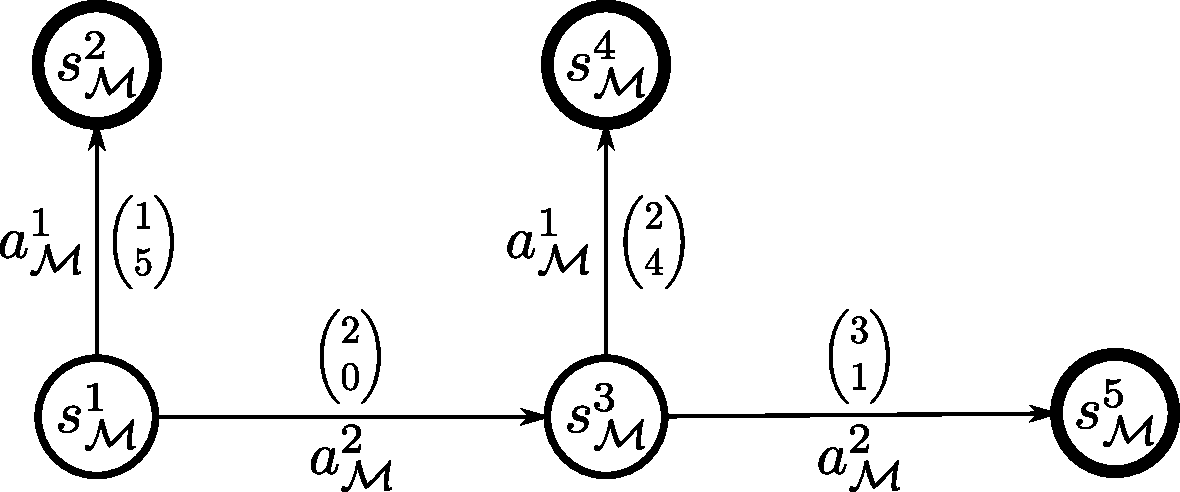
\includegraphics[width=0.8\textwidth]{figures/ch2/example_momdp.pdf} 
        \caption[An example MOMDP $\bfcl{M}$.]{An example MOMDP $\bfcl{M}$, where $s_0=s_{\cl{M}}^1$, the finite horizon is $H=2$ and terminal states are marked with thicker borders. This particular MOMDP is deterministic, so all transition probabilities are one.}
        \label{fig:2:momdp_eg}
    \end{figure}

    Now multi-objective trajectories are defined:
    \begin{defn}
        \label{def:2:mo_trajectory}
        A \textnormal{multi-objective trajectory} $\tau$, is a sequence of state, action and vector rewards, that is induced by a policy $\pi$ and MOMDP $\bfcl{M}$ pair. Let the trajectory be $\bff{\tau} = (s_0, a_0, \bff{r}_0, s_1, a_1, \bff{r}_1, ..., s_{H-1}, a_{H-1}, \bff{r}_{H-1}, s_H)$, where $a_t \sim \pi(\cdot|s_t)$, $\bff{r}_t=\bff{R}(s_t,a_t)$ and $s_{t+1} \sim p(\cdot|s_t,a_t)$. 
        
        The notations used for single-objective trajectories (Definition \ref{def:2:trajectory}) will also be used for multi-objective trajectories too. Such as, $\bff{\tau}\sim\pi$ for sampling trajectories using policies, and $\bff{\tau}_{i:j}$ for truncated trajectories.
    \end{defn}

    Similarly, multi-objective variants of the (Q-)value of a policy are defined:    
    \begin{defn}
        \label{def:2:mo_value}
        \label{def:2:mo_q_value}
        The \textnormal{multi-objective value} of a policy $\pi$ from state $s$ at time $t$ is:
        \begin{align}
            \bff{V}^{\pi}(s;t) = \bb{E}_{\bff{\tau}\sim\pi}\left[\sum_{i=t}^{H-1} \bff{r}_t \Bigg| s_t=s \right]. \label{eq:2:mo_value_fn_def}
        \end{align} 

        The \textnormal{multi-objective Q-value} of a policy $\pi$, from state $s$, with action $a$, at time $t$ is:
        \begin{align}
            \bff{Q}^{\pi}(s,a;t) = \bff{R}(s,a) + \bb{E}_{s'\sim p(\cdot|s,a)} [\bff{V}^{\pi}(s';t+1)]. \label{eq:2:mo_q_value_fn_def}
        \end{align} 
    \end{defn}

    In the corresponding point of the single-objective reinforcement learning section (Section \ref{sec:2-3-rl}), the the optimal (Q-)value functions and the objective of single-objective reinforcement learning were defined. However, in a multi-objective setting there is no longer a \textit{total ordering} over values, and so there maybe be multiple vectors that could be ``optimal''. For example, consider two vectors $\bff{u},\bff{v}\in\bb{R}^2$ which are such that $u_1 > v_1$ and $u_2 < v_2$. To resolve this issue, a \textit{utility function} or \textit{scalarisation function} is used to map multi-objective values to scalar values.

    \begin{defn}
        \label{def:2:simplex}
        \label{def:2:weight}
        \label{def:2:context}
        The \textnormal{($D$-dimensional) Simplex} consists of the set of $D$-dimensional vectors, whose entries are non-negative and sum to one. More formally, the $D$ dimensional simplex is 
        \begin{align}
            \Delta^D = \{\bff{w}\in\bb{R}^D|w_i > 0, \sum_i w_i = 1\}. \label{eq:2:simplex_def}
        \end{align}

        The elements of the $D$-dimensional Simplex will be referred to as \textnormal{weight vectors} (or just \textnormal{weights}) in this thesis, as they will be used to specify preferences over the $D$ dimensions of the reward function.
    \end{defn}

    \begin{defn}
        \label{def:2:utility_fn}
        \label{def:2:scalarisation_fn}
        A \textnormal{utility function} (or \textnormal{scalarisation function}) $u:\mathbb{R}^D\times\Delta^D \rightarrow \bb{R}$ is used to map from a multi-objective value $\bff{v}\in\bb{R}^D$ and a weighting over the objectives $\bff{w}\in\Delta^D$ to a scalar value. That is, according to the utility function $u(\cdot;\bff{w})$ the multi-objective value $\bff{v}$ is mapped to the scalar value $u(\bff{v};\bff{w})$.
    \end{defn}

    Of particular interest in this thesis is the \textit{linear utility function} where the scalar value takes the form of a dot-product:
    \begin{defn}
        \label{def:2:linear_utility_fn}
        \label{def:2:linear_scalarisation_fn}
        The \textnormal{linear utility function} $u_{\lin}$ is the utility function defined by:
        \begin{align}
            u_{\lin}(\bff{v};\bff{w}) = \bff{w}^\top \bff{v}. \label{eq:2:linear_utility_fn_def}
        \end{align}
    \end{defn}

    Equipped with a utility function and a weight vector any set of multi-objective values can be mapped to scalars and ordered. A policy is \textit{possibly optimal}, or \textit{undominated}, with respect to utility function $u$ if it achieves a maximal utility for some weight $w\in\Delta^D$. In contrast, a policy is \textit{dominated} if for every weight there is another policy that achieves a better utility. 
    
    Let $\Pi$ be the set of all possible policies for a given MOMDP. When constructing a solution set, a subset of $\Pi$, it makes sense that it should not contain any dominated policies. This leads to the first notion of a solution set, called an \textit{undominated set}, consisting of all undominated policies:
    \begin{defn}
        \label{def:2:undominated_set}
        \label{def:2:convex_hull}
        The \textnormal{undominated set} of policies $U(\Pi;u)\subseteq\Pi$, with respect to a utility function $u$,  is the set of policies for which there is a weight vector $\bff{w}\in\Delta^D$ where the utility (scalarised value) is maximised: 
        \begin{align}
            U(\Pi;u) = \left\{\pi\in\Pi\ \big|\ \exists \bff{w}\in\Delta^D. \forall \pi'\in\Pi: u(\bff{V}^{\pi}(s_0;0);\bff{w}) \geq u(\bff{V}^{\pi'}(s_0;0);\bff{w}) \right\}. \label{eq:2:undominated_set_def}
        \end{align}

        In particular, the \textnormal{convex hull} of policies $CH(\Pi)$ is the undominated set with respect to the linear utility function $u_{\lin}$. That is $CH(\Pi)=U(\Pi;u_{\lin})$.
    \end{defn}    

    \quest{How do you feel about removing the timestep in the value functions in this section too? So it can be $\bff{V}^\pi(s)$ rather than $\bff{V}^\pi(s;t)$? I think it would make some definitions like undominated sets a bit cleaner. Alternatively, maybe I should write it $u_{\bff{w}}$.}
    
    When computing solutions sets, it is often useful to first compute the multi-objective values that could be obtained, and then later use the data structures used by the algorithm to read out the selected policy. This thesis will refer to the set of values obtained by a set of policies as a \textit{value set}:
    \begin{defn}
        \label{def:2:mo_value_set}
        The \textnormal{(multi-objective) value set} with respect to a set of policies $\Pi'\subseteq\Pi$ is defined as $\valset(\Pi') = \{\bff{V}^{\pi}(s_0;0) | \pi \in \Pi'\}$.
    \end{defn}

    Undominated sets often have an infinite cardinality, and as such are infeasible to compute. However, in undominated sets there are often many reduntant policies that obtain the same scalarised values. Instead of computing an undominated set, it is more feasible to compute a \textit{coverage sets} which contain at least one policy that maximises the scalarised value given any weight vector $\bff{w}$:
    \begin{defn}
        \label{def:2:coverage_set}
        \label{def:2:convex_coverage_set}
        A set $CS(\Pi;u)\subseteq U(\Pi)$, is a \textnormal{coverage set} with respect to a utility function $u$, if for every weight vector $\bff{w}\in\Delta^D$, there is a policy $\pi\in CS(\Pi;u)$ that maximises the value of $u(\cdot;\bff{w})$. That is, for $CS(\Pi;u)$ to be a coverage set, the following statement must be true:
        \begin{align}
            \forall \bff{w}\in\Delta^D. \exists \pi\in CS(\Pi;u). \forall \pi'\in\Pi: u(\bff{V}^{\pi}(s_0;0);\bff{w}) \geq u(\bff{V}^{\pi'}(s_0;0);\bff{w}). \label{cond:coverage_set}
        \end{align}

        Again, in particular, any set $CCS(\Pi)$ is a \textnormal{convex coverage set} if it is a coverage set with respect to the linear utility function $u_{\lin}$. 
    \end{defn}

    Note that it is still possible for there to be multiple coverage sets. Algorithms that compute convex coverage sets typically compute a unique minimal convex coverage set that contains no redundant policies, that is, each policy has some weight for which it uniquely gives an optimal solution in the set.
    \begin{defn}
        \label{def:2:min_convex_coverage_set}
        A set $CCS_{\min}(\Pi)\subseteq CH(\Pi)$ is minimal if the following holds
        \begin{align}
         \forall \pi\in CCS_{\min}(\Pi). \exists \bff{w}\in\Delta^D. \forall \pi'\in CCS_{\min}(\Pi)-\{\pi\}. u_{\lin}(\bff{V}^{\pi}(s_0;0);\bff{w}) > u_{\lin}(\bff{V}^{\pi'}(s_0;0);\bff{w}).
        \end{align}
    \end{defn} 

    Now the geometry of convex coverage sets is considered, to see how something like $\valset(CCS_{\min}(\Pi))$ can be computed. Firstly, any multi-objective values that obtain the same linear utility will lie on a hyperplane, whose normal is the weight vector used in the linear utility function (see (a) in Figure \ref{fig:2:convex_hull_geometry}). As a result, the values of the convex hull, $\valset(CH(\Pi))$ lie on a \textit{geometric (partial) convex hull} (see (b) in Figure \ref{fig:2:convex_hull_geometry}). Moreover, any points in $\valset(CH(\Pi))$ that lie on the edge of the geometric convex hull are redundant, as the values corresponding to the neighbouring vertices of geometric convex hull will always achieve the same or greater utility (see (c) in Figure \ref{fig:2:convex_hull_geometry}).

    Because of the ambiguity between the convex hull of policies, and the geometric convex hulls of values, this thesis will refer to any value set that forms a geometric convex hull as a \textit{convex hull value set} (CHVS) and will refer to the set $\valset(CCS_{\min}(\Pi))$ as the \textit{optimal convex hull value set}. \quest{should I make this paragraph a definition to emphasise it a bit more?}

    \begin{figure}
        \centering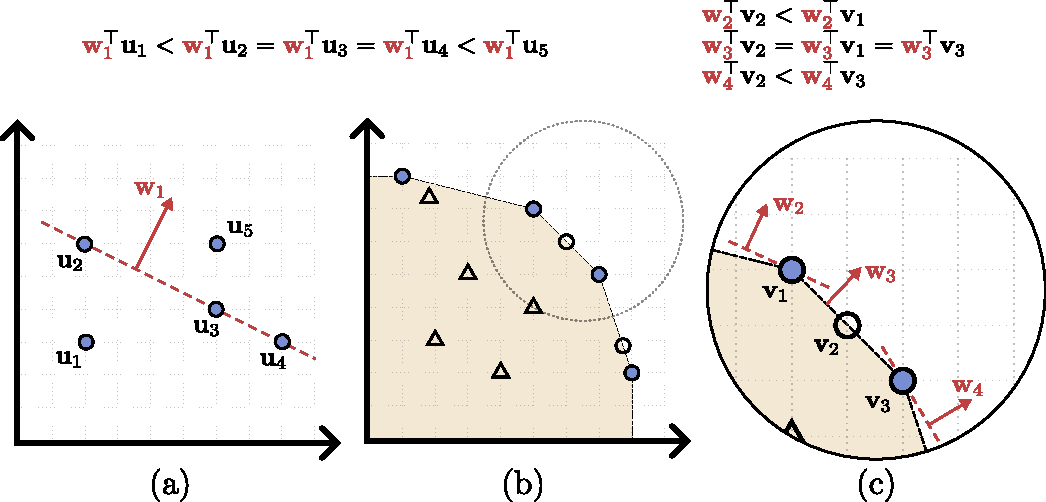
\includegraphics[width=1.0\textwidth]{figures/ch2/ch_geometry.pdf} 
        \caption[The geometry of convex coverage sets.]{The geometry of convex coverage sets, shown with $D=2$. In each images the points depicted correspond to a value set $\valset(\Pi')$, for some set of policies $\Pi'$. (a) demonstrates that values ($\bff{u}_2$,$\bff{u}_3$,$\bff{u}_4$) obtaining the same utility lie on a hyperplane. Moving in the direction of the weight vector increases the utility ($\bff{u}_5$) and likewise moving in the opposite direction decreases utility ($\bff{u}_1$); (b) circles correspond to values that are on the convex hull, so form the set $\valset(CH(\Pi'))$, the blue circles form the minimal convex coverage set, $\valset(CCS_{\min}(\Pi'))$, and triangles are not part of the convex hull. All of the unfilled shapes would be pruned by \cprune (Equation (\ref{eq:2:cprune_def})); (c) shows a magnification of (b) with additional labels, it shows that the value $\bff{v}_2$ is redundant because one of $\bff{v}_1$ or $\bff{v}_3$ will achieve an equal or greater utility. Additionally, is shows $\bff{w}_2$ and $\bff{w}_4$ which are weights that the values $\bff{v}_1$ and $\bff{v}_3$ uniquely maximise the utility within $\valset(\Pi')$}
        \label{fig:2:convex_hull_geometry} 
    \end{figure}

    Given a value set, the \cprune\ewe operation removes any vectors that are dominated or redundant. That is, for every vector that remains after the pruning operation, there is some weight for which it \textit{uniquely} gives the maximal utility for. Given set of vectors $\bfcl{V}$ it is defined as:
    \begin{align}
        \cprune(\bfcl{V}) = \{\bff{v}\in\bfcl{V} | \exists \bff{w}\in\Delta^D. \forall \bff{v}'\in\bfcl{V}-\{\bff{v}\}. \bff{w}^\top \bff{v} > \bff{w}^\top \bff{v}' \}. \label{eq:2:cprune_def}
    \end{align}

    Note that the \cprune\ewe operator computes the values of a minimal convex coverage set, that is, for some set of policies $\Pi'$ the $\cprune$ operation satisfies $\cprune(\valset(\Pi')) = \valset(CCS_{\min}(\Pi'))$. \cprune\ewe can be implemented using \textit{linear programming} \cite{cccs}, and an example of its operation on a set of vectors can be seen in (b) of Figure \ref{fig:2:convex_hull_geometry}, where \cprune\ewe would prune all points but the blue circles.




    \subsection{Convex Hull Value Iteration}
    \label{sec:2-5-1-chvi}

        Convex Hull Value Iteration (CHVI) \cite{chvi} is a tabular dynamic programming algorithm similar to Value Iteration (Section \ref{sec:2-3-rl}) that will compute optimal convex hull value sets. In CHVI the value estimates of Value Iteration are replaced by CHVSs, which are estimates of the optimal CHVS. These estimates will be denoted $\Vchvi(s;t)$ and $\Qchvi(s,a;t)$.

        Firstly, to define a multi-objective version of Value Iteration, an arithmetic over vector sets needs to be defined. An example of the following arithmetic is given in Figure \ref{fig:2:vectorset_arithmetic} Given the vector sets $\bfcl{U}$ and $\bfcl{V}$, define multiplication by a scalar $s$, addition with a vector $\bff{x}$ and addition between sets as follows:
        \begin{align}
            \bff{x} + s\bfcl{V} &= \{\bff{x} + s\bff{v} | \bff{v}\in\bfcl{V} \} \label{eq:2:vector_set_arithmetic_one} \\
            \bfcl{U} + \bfcl{V} &= \{ \bff{u}+\bff{v} | \bff{u}\in\bfcl{U}, \bff{v}\in\bfcl{V} \}. \label{eq:2:vector_set_arithmetic_two} 
        \end{align}

        \begin{figure}
            \centering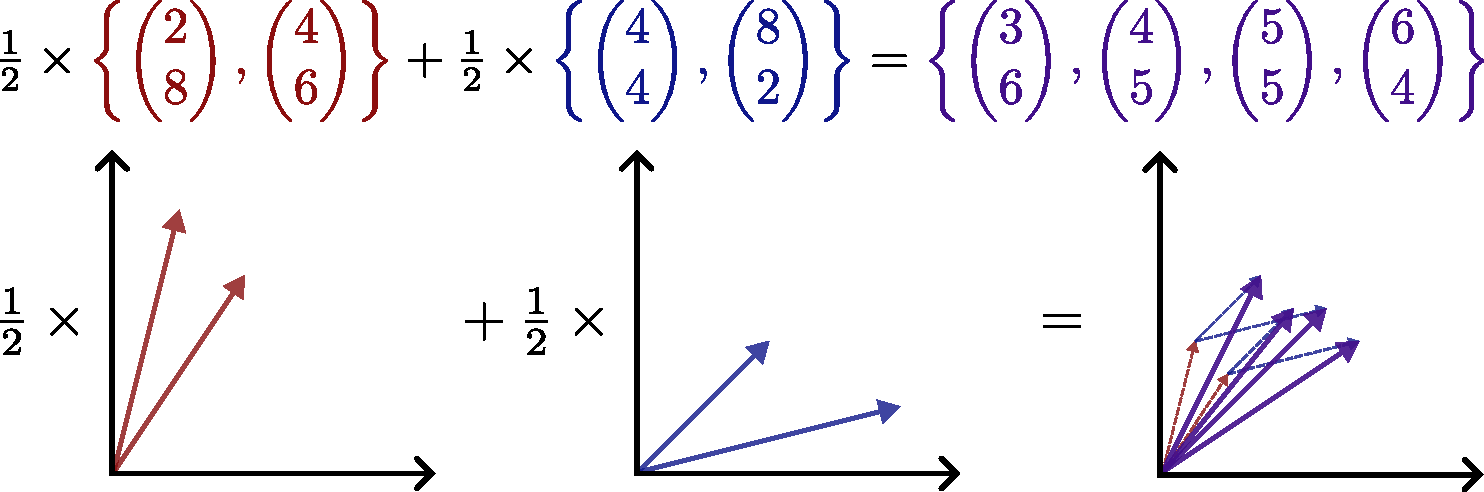
\includegraphics[width=1.0\textwidth]{figures/ch2/ch_arithmetic.pdf} 
            \caption[An example of arithmetic over vector sets.]{An example of arithmetic over vector sets. Two vector sets are shown in red and blue, which are multiplied by $\frac{1}{2}$ using Equation (\ref{eq:2:vector_set_arithmetic_one}), and then added using Equation (\ref{eq:2:vector_set_arithmetic_two}). On the right the resulting vector set is shown in purple, which are the sum of appropriately scaled red and blue vectors.}
            \label{fig:2:vectorset_arithmetic}
        \end{figure}

        Now to define the multi-objective Bellman backups used in CHVI, let $\Vchvi^0(s;t) = \{ \bff{0} \}$, where $\bff{0}=(0,...,0)\in\bb{R}^D$. The CHVI backups are then:
        \begin{align}
            \Vchvi^{k+1}(s;t) &= \cprune \left( \bigcup_{a\in\cl{A}} \Qchvi^{k+1}(s,a;t) \right), \label{eq:2:chvi_v_backup} \\
            \Qchvi^{k+1}(s,a;t) &= \bb{E}_{s'\sim p(\cdot|s,a)} [\bff{R}(s,a) + \Vchvi^k(s';t+1)]. \label{eq:2:chvi_q_backup}
        \end{align}
        
        This again parallels the Bellman backups use in single-objective Value Iteration, where the max operation is replaced by the \cprune\ewe operation over the set of achievable values from the current state $s$: $\bigcup_{a\in\cl{A}} \Qchvi^{k+1}(s,a;t)$.
        
        Once the algorithm has terminated, and a weight $\bff{w}$ is provided, a policy can be extracted by computing scalar Q-values from the CHVSs \cite{chvi}:
        \begin{align}
            Q_{\bff{w}}(s,a;t) = \max_{\bff{q}\in\Qchvi(s,a;t)} \bff{w}^\top \bff{q}, \label{eq:2:chvi_scalar_q_fn} \\
            \pichvi(s;t,\bff{w}) = \argmax_{a\in\cl{A}} Q_{\bff{w}}(s,a;t). \label{eq:2:chvi_policy}
        \end{align}

        If the user would rather select a particular value from the CHVS, say $\bff{v}\in\Vchvi(s_0;0)$, rather than provide a weight, one can be computed. Let $\bff{v}_\bot$ be a \textit{reference point}, defined at each index as:
        \begin{align}
            (v_{\bot})_i = \min \{v'_i | \bff{v}'\in\Vchvi(s_0;0) \}. \label{eq:2:chvi_ref_point}
        \end{align} 

        The vector that runs from $\bff{v}_\bot$ to $\bff{v}$ provides an appropriate weighting over objectives for which $\bff{v}$ will produce the largest utility out of $\hat{\bfcl{V}}(s_0;0)$, as is demonstrated in Figure \ref{fig:2:convex_hull_extract_policy_weight}. Hence, to extract a policy that achieves the value $\bff{v}$ the weight $\bff{w}$ should be set to:
        \begin{align}
            \bff{w} = \frac{\bff{v}-\bff{v}_\bot}{\Vert\bff{v}-\bff{v}_\bot\Vert_2}, \label{eq:2:chvi_extract_value_weight}
        \end{align}

        and then follow $\pichvi(s;t,\bff{w})$ as defined in Equation (\ref{eq:2:chvi_policy}).
        
        \begin{figure}
            \centering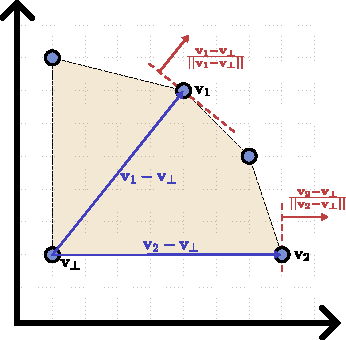
\includegraphics[width=0.5\textwidth]{figures/ch2/ch_extract_policy_weight.pdf} 
            \caption[A visualisation, reusing the convex hull from Figure \ref{fig:2:convex_hull_geometry}, demonstrating how to compute a weight vector that can be used to extract a specific value from a vector set.]{A visualisation, reusing the convex hull from Figure \ref{fig:2:convex_hull_geometry}, demonstrating how to compute a weight vector that can be used to extract a specific value from a vector set. The hyperplane running through $\bff{v}_i$ with normal $\bff{w}_i=\frac{\bff{v}_i-\bff{v}_\bot}{\Vert\bff{v}_i-\bff{v}_\bot\Vert_2}$ is tangential to the geometric convex hull. Hence $\bff{v}_i$ is the optimal value for the weight $\bff{w}_i$ and following the CHVI policy in Equation (\ref{eq:2:chvi_policy}) will give the desired value $\bff{v}_i$.}
            \label{fig:2:convex_hull_extract_policy_weight} 
        \end{figure}











\section{Sampling From Catagorical Distributions}
\label{sec:2-6-sampling}
    
    \quest{Maybe heres a good time to ask about some notation stuff. So I used $m$ in MABs section, and I reuse it here. Is that ok? I was trying to keep as much notation unique as possible, but noticed I've reused a couple variables. I was hoping its ok because I'm using them ``locally''.}

    Some of the work in this thesis will involve sampling from catagorical distributions, and sometimes it will be helpful to do so efficiently, as in Chapter \ref{ch:4-dents}. Let $f:\{C_1,...,C_m\}\rightarrow[0,1]$ be the probability mass function of a catagorical distribution with $m$ categories. Suppose that we want to sample $c\sim f$. A naive method to sample from $f$ will take $O(m)$ time, where a continuous uniform random value is sampled, $u\sim\textnormal{Uniform}(0,1)$, and $f$ is linearly scanned until a probability mass of $u$ has been passed. See Listing \ref{lst:2:naive_sample} for psuedocode of the naive method.

    \begin{Listing}
        \begin{lstlisting}
def sample_catagorical($f$):
    threshold $\sim \textnormal{Uniform}(0,1)$
    i = 0
    accumulated_mass = 0
    while (accumulated_mass < threshold):
        i += 1
        accumulated_mass += $f($i$)$
    return i
        \end{lstlisting}
        \caption{Psuedocode for naively sampling from a catagorical distribution.}
        \label{lst:2:naive_sample}
    \end{Listing}

    However, the \textit{alias method} \cite{alias_method_one,alias_method_two} can instead be used to sample from a catagorical distribution. The alias method uses $O(m)$ preprocessing time to construct an \textit{alias table}, and after can sample from $f$, using the table, in $O(1)$ time. An alias table consists of $m$ entries, accounting for an $m$th of the probability mass of $f$. Each entry takes the form $(c_0,c_1,\thresh)$, where $c_0,c_1\in\{C_1,...,C_m\}$ are categories and $\thresh\in[0,1]$ gives the ratio of the $\frac{1}{m}$ probability mass to assign to $c_0$ and $c_1$. Sampling from the alias table can be performed by sampling two random numbers, one to index into the table and one to compare against $\thresh$, from which $c\sim f$ can be returned by looking it up in the table. Listing \ref{lst:2:alias_table_sample} gives psuedocode for sampling from an alias table, and Figure \ref{fig:2:alias_table_eg} visualises the construction and sampling of an alias table.

    \begin{Listing}
        \begin{lstlisting}
def sample_from_alias_table(alias_table):
    index $\sim \textnormal{Uniform}(\{1,...,m\})$
    $(c_0,c_1,\thresh)$ = alias_table[index]
    $u \sim \textnormal{Uniform}(0,1)$
    if ($u <= \thresh$):
        return $c_0$ 
    return $c_1$
        \end{lstlisting}
        \caption{Psuedocode for sampling from an alias table.}
        \label{lst:2:alias_table_sample}
    \end{Listing}

        
    \begin{figure}
        \centering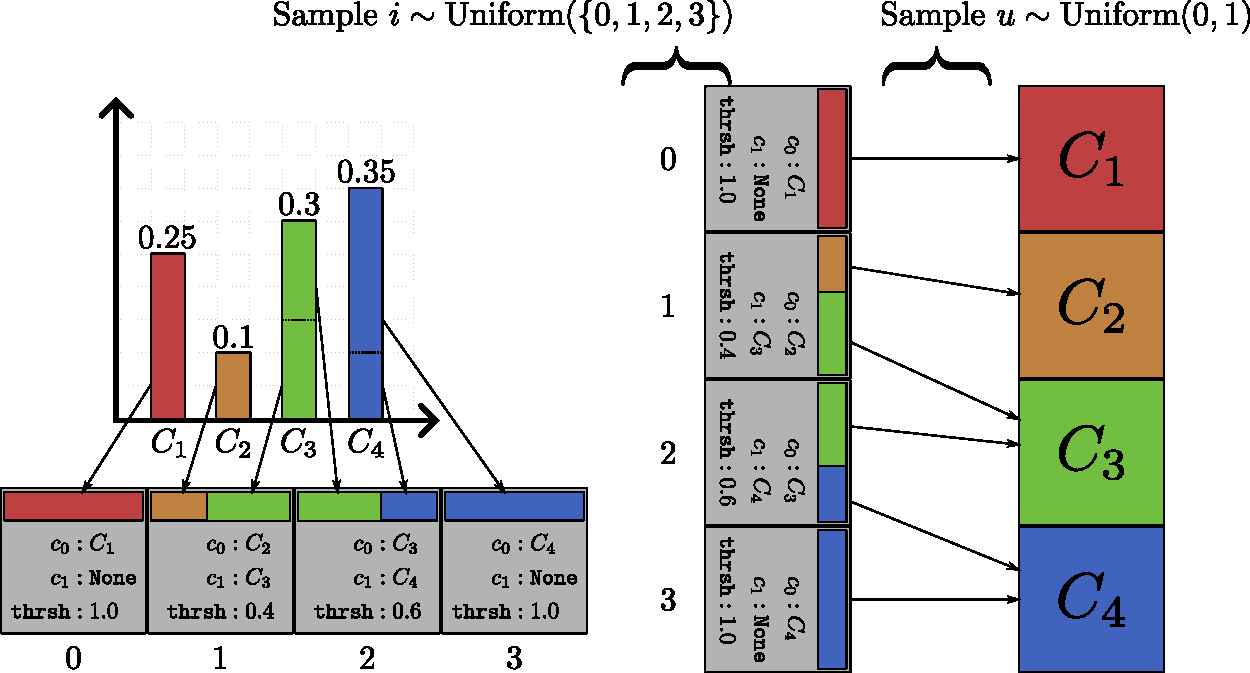
\includegraphics[width=0.9\textwidth]{figures/ch2/alias_table.pdf} 
        \caption[Example of building and sampling from an alias table.]{Example of building and sampling from an alias table, on a distribution with four categories. Left: shows how the probability mass is split into the four entries of the table. Right: shows how two random variables can be used to sample from the table in $O(1)$ time, where $i$ is used to index into the table, and $u$ is used to compare with \thresh\ewe and decide which of the two arrows from the entry to follow.}
        \label{fig:2:alias_table_eg} 
    \end{figure}

    \citet{alias_method_two} proves that an alias table can always be constructed from an arbitrary catagorical distribution, such that the probability of sampling any catagory from the alias table is identical to the probability of sampling it from the original probability mass function. 

    Psuedocode for constructing an alias table is given in Listing \ref{lst:2:alias_table_construct}, following \cite{alias_method_one,alias_method_two}. An alias table can be constructed by keeping two sets of categories, one set for ``big'' categories that currently have more than $\frac{1}{m}$ mass to be added to the table, and one for ``small'' catagories that have at most $\frac{1}{m}$ mass left to be added to the table. To create a new entry in the table, take one category from the small set, and take a category from the big set to complete the remainder of the $\frac{1}{m}$ mass that the small set didn't fill. After creating a new entry, move the big category to the little set if it no longer has more than $\frac{1}{m}$ mass to be added. 

    \begin{Listing}
        \begin{lstlisting}
def build_alias_table($f$):
    # lists of categories and mass remaining
    small = []
    big = []
    
    # fill big and small lists
    for $c$ in $f$:
        if $f(c) > \frac{1}{m}$:
            big.append($(c,f(c))$)
        else:
            small.append($(c,f(c))$)

    # construct alias table
    alias_table = []
    while len(small) > 0:
        # create entry
        $c_0$, c0_mass_remaining = small.pop()
        if mass_remaining == $\frac{1}{m}$:
            alias_table.append($(c_0,\text{None},1.0)$)
            continue
        $c_1$, c1_mass_remaining = big.pop()

        # add entry to table (accounting for 1/mth of total mass)
        thrsh = $m$ * c0_mass_remaining
        alias_table.append($(c_0,c_1,$thrsh$)$)

        # put c1 back in lists appropriately
        c1_mass_remaining -= c0_mass_remaining
        if c1_mass_remaining > $\frac{1}{m}$:
            big.append($(c_1,$c1_mass_remaining$)$)
        else:
            small.append($(c_1,$c1_mass_remaining$)$)
        
    return alias_table
        \end{lstlisting}
        \caption{Psuedocode for constructing an alias table.}
        \label{lst:2:alias_table_construct}
    \end{Listing}





